\documentclass[twoside,11pt,letter]{article}
\usepackage[margin=1in]{geometry}
\usepackage{amsmath, amssymb, amsthm}
\usepackage{bm}
\usepackage{hyperref}
\usepackage{enumitem}
\usepackage[dvipsnames]{xcolor}
\usepackage{setspace}

\hypersetup{
	colorlinks=true,
	linkcolor=MidnightBlue,
	urlcolor=MidnightBlue,
	citecolor=MidnightBlue
}

\setstretch{1.08}

\usepackage{times}
\usepackage{amsmath}
\usepackage{amsfonts}
\usepackage{amssymb}
\usepackage{amsthm}
\usepackage{makeidx} 
\usepackage{graphicx}
\usepackage{mathrsfs}
\usepackage{tabularx}
\usepackage{caption}
\usepackage{bbold}
\usepackage{color}
\usepackage{fancybox}
\usepackage{verbatim}
\usepackage{hyperref}
\usepackage{tikz}
\usepackage{float}
\usepackage{url}
\usetikzlibrary{arrows,automata}
\usetikzlibrary{trees}
\usetikzlibrary{shadows}
\usepackage[framemethod=TikZ]{mdframed}
\usepackage{mdframed}
\usepackage[ruled,vlined]{algorithm2e}
\usepackage{booktabs}
\usepackage{youngtab}
\mdfdefinestyle{theorem}{%
	linecolor=black,
	outerlinewidth=.5pt,
	roundcorner=5pt,
	innertopmargin=.5\baselineskip,
	innerbottommargin=.75\baselineskip,
	innerrightmargin=20pt,
	innerleftmargin=20pt,
	backgroundcolor=green!20,
	shadow=true,
	shadowcolor=green!20}
\mdfdefinestyle{algo}{%
	linecolor=black,
	outerlinewidth=.5pt,
	roundcorner=5pt,
	innertopmargin=.5\baselineskip,
	innerbottommargin=.75\baselineskip,
	innerrightmargin=10pt,
	innerleftmargin=10pt,
	backgroundcolor=yellow!20,
	shadow=true,
	shadowcolor=yellow!20}
\mdfdefinestyle{example}{%
	linecolor=black,
	outerlinewidth=.5pt,
	leftline = false,
	rightline = false,
	%roundcorner=5pt,
	innertopmargin=.5\baselineskip,
	innerbottommargin=.75\baselineskip,
	innerrightmargin=10pt,
	innerleftmargin=10pt,
	backgroundcolor=white}

\def\bC{\mathbb{C}}
\def\bH{\mathbb{H}}
\def\bI{\mathbb{I}}
\def\bJ{\mathbb{J}}
\def\bK{\mathbb{K}}
\def\bN{\mathbb{N}}
\def\bP{\mathbb{P}}
\def\bR{\mathbb{R}}
\def\bS{\mathbb{S}}
\def\bZ{\mathbb{Z}}
\def\b1{\mathbb{1}}

\def\bfA{\mathbf{A}}
\def\bfb{\mathbf{b}}
\def\bfB{\mathbf{B}}
\def\bfC{\mathbf{C}}
\def\bfD{\mathbf{D}}
\def\bfE{\mathbf{E}}
\def\bfF{\mathbf{F}}
\def\bfG{\mathbf{G}}
\def\bfH{\mathbf{H}}
\def\bfJ{\mathbf{J}}
\def\bfK{\mathbf{K}}
\def\bfL{\mathbf{L}}
\def\bfM{\mathbf{M}}
\def\bfN{\mathbf{N}}
\def\bfP{\mathbf{P}}
\def\bfQ{\mathbf{Q}}
\def\bfR{\mathbf{R}}
\def\bfS{\mathbf{S}}
\def\bfU{\mathbf{U}}
\def\bfx{\mathbf{x}}

\def\e1{\mathsf{1}}
\def\eD{\mathsf{D}}
\def\eE{\mathsf{E}}
\def\eF{\mathsf{F}}
\def\eH{\mathsf{H}}
\def\eI{\mathsf{I}}
\def\eM{\mathsf{M}}
\def\eP{\mathsf{P}}
\def\eQ{\mathsf{Q}}
\def\eS{\mathsf{S}}
\def\eT{\mathsf{T}}
\def\eQj{\mathsf{Q}_j}
\def\eQk{\mathsf{Q}_k}
\def\eQl{\mathsf{Q}_l}
\def\eQmn{\mathsf{Q}_{mn}}
\def\en{\mathsf{n}}
\def\ep{\mathsf{p}}
\def\eq{\mathsf{q}}

\def\tT{\mathtt{T}}

\def\fa{{\mathfrak{a}}}
\def\fb{{\mathfrak{b}}}
\def\fc{{\mathfrak{c}}}
\def\fd{{\mathfrak{d}}}
\def\fe{{\mathfrak{e}}}
\def\ff{{\mathfrak{f}}}
\def\fg{{\mathfrak{g}}}
\def\fh{{\mathfrak{h}}}
\def\fl{{\mathfrak{l}}}
\def\fm{{\mathfrak{m}}}
\def\fn{{\mathfrak{n}}}
\def\fo{{\mathfrak{o}}}
\def\fp{{\mathfrak{p}}}
\def\fr{{\mathfrak{r}}}
\def\fs{{\mathfrak{s}}}
\def\ft{{\mathfrak{t}}}
\def\fv{{\mathfrak{v}}}
\def\fw{{\mathfrak{w}}}
\def\fz{{\mathfrak{z}}}
\def\fA{{\mathfrak{A}}}
\def\fB{{\mathfrak{B}}}
\def\fC{{\mathfrak{C}}}
\def\fD{{\mathfrak{D}}}
\def\fF{{\mathfrak{F}}}
\def\fG{{\mathfrak{G}}}
\def\fH{{\mathfrak{H}}}
\def\fI{{\mathfrak{I}}}
\def\fL{{\mathfrak{L}}}
\def\fM{{\mathfrak{M}}}
\def\fN{{\mathfrak{N}}}
\def\fO{{\mathfrak{O}}}
\def\fP{{\mathfrak{P}}}
\def\fR{{\mathfrak{R}}}
\def\fS{{\mathfrak{S}}}
\def\fT{{\mathfrak{T}}}
\def\fU{{\mathfrak{U}}}
\def\fV{{\mathfrak{V}}}
\def\fX{{\mathfrak{X}}}
\def\fW{{\mathfrak{W}}}
\def\fZ{{\mathfrak{Z}}}

\def\cA{\mathcal{A}}
\def\cB{\mathcal{B}}
\def\cC{\mathcal{C}}
\def\cD{{\mathcal{D}}}
\def\cE{{\mathcal{E}}}
\def\cF{{\mathcal{F}}}
\def\cG{{\mathcal{G}}}
\def\cH{{\mathcal{H}}}
\def\cI{{\mathcal{I}}}
\def\cJ{{\mathcal{J}}}
\def\cK{{\mathcal{K}}}
\def\cL{\mathcal{L}}
\def\cM{\mathcal{M}}
\def\cN{\mathcal{N}}
\def\cO{{\mathcal{O}}}
\def\cP{{\mathcal{P}}}
\def\cQ{{\mathcal{Q}}}
\def\cR{{\mathcal{R}}}
\def\cS{{\mathcal{S}}}
\def\cT{{\mathcal{T}}}
\def\cU{{\mathcal{U}}}
\def\cV{{\mathcal{V}}}
\def\cX{{\mathcal{X}}}
\def\cY{{\mathcal{Y}}}
\def\cZ{{\mathcal{Z}}}

\def\sC{{\mathscr{C}}}
\def\sD{{\mathscr{D}}}
\def\sE{{\mathscr{E}}}
\def\sF{{\mathscr{F}}}
\def\sG{{\mathscr{G}}}
\def\sH{{\mathscr{H}}}
\def\sL{{\mathscr{L}}}
\def\sO{{\mathscr{O}}}
\def\sS{{\mathscr{S}}}
\def\sX{{\mathscr{X}}}
\def\sY{{\mathscr{Y}}}
\def\sZ{{\mathscr{Z}}}

\def\tc{{\text{c}}}
\def\tf{{\text{f}}}

\def\cov{\mathsf{Cov}}
\def\corr{\mathsf{Corr}}
\def\var{\mathsf{Var}}
\def\prob{\mathsf{prob}}
\def\dom{\mathsf{dom}}
\def\sign{\mathsf{sign}}
\def\rank{\mathsf{rank}}
\def\e1{\mathsf{1}}

\def\ofa{(a)}
\def\ofb{(b)}
\def\ofi{(i)}
\def\ofK{(K)}
\def\ofp{(p)}
\def\ofr{(r)}
\def\ofs{(s)}
\def\ofS{(S)}
\def\oft{(t)}
\def\ofT{(T)}
\def\ofT{(T)}
\def\ofu{(u)}
\def\ofv{(v)}
\def\ofw{(w)}
\def\ofx{(x)}
\def\ofy{(y)}
\def\ofz{(z)}
\def\of0{(0)}
\def\oftau{(\tau)}

\def\d{\partial}
\def\tr{\mathrm{tr}}
\def\id{\mathrm{I}}
\def\bfId{\mathbf{I}}
\def\bfNabla{\mathbf{\nabla}}
\def\bf0{\mathbf{0}}
\def\cp1{\mathbb{CP}^1}
\def\matn{\mathrm{Mat}_n(\bR)}
\def\symn{\mathrm{Sym}_n(\bR)}
\def\Gr{\mathrm{Gr}}
\def\arg{\mathrm{arg}}
\def\im{\mathrm{Im}}
\def\re{\mathrm{Re}}
\def\argmax{\mathop{\arg\max}}
\def\Exp{\mathrm{Exp}}

\def\parP{\mathrm{PAR}}
\def\pv{\textsf{PV}}
\def\df{\mathrm{Df}}

\def\erf{\mathrm{erf}}

%Elliptic functions
\def\am{\mathrm{am}}
\def\sn{\mathrm{sn}}
\def\cn{\mathrm{cn}}
\def\dn{\mathrm{dn}}

%Normalized Hermite polynomials
\def\Her{\mathrm{He}}
\def\her{h}

\newtheorem{theorem}{Theorem}[section]
%\newtheorem{algorithm}[theorem]{Algorithm}
\newtheorem{assumption}[theorem]{Assumption}
\newtheorem{axiom}[theorem]{Axiom}
\newtheorem{case}[theorem]{Case}
\newtheorem{claim}[theorem]{Claim}
\newtheorem{conclusion}[theorem]{Conclusion}
\newtheorem{condition}[theorem]{Condition}
\newtheorem{conjecture}[theorem]{Conjecture}
\newtheorem{corollary}[theorem]{Corollary}
\newtheorem{criterion}[theorem]{Criterion}
\theoremstyle{definition}
\newtheorem{definition}[theorem]{Definition}
\theoremstyle{definition}
\newtheorem{example}[theorem]{Example}
\newtheorem{exercise}[theorem]{Exercise}
\newtheorem{lemma}[theorem]{Lemma}
\newtheorem{notation}[theorem]{Notation}
\newtheorem{problem}[theorem]{Problem}
\newtheorem{proposition}[theorem]{Proposition}
%\newtheorem{remark}[theorem]{Remark}
\newtheorem{solution}[theorem]{Solution}
\newtheorem{summary}[theorem]{Summary}

%\newenvironment{proof}[1][Proof]{\noindent\textbf{#1:} }{\ \rule{0.5em}{0.5em}}
%\newenvironment{example}[1][Example]{\vskip.2cm\noindent\textbf{#1}. }{\ \vskip.2cm}

\newenvironment{remark}[1][Remark.]{\begin{trivlist}
		\item[\hskip \labelsep {\bfseries #1}]}{\end{trivlist}}

\DeclareMathOperator{\diag}{diag}
\DeclareMathOperator{\ad}{ad}


\pagestyle{myheadings} \markboth{A. Deep, A. Lesniewski, O. Missaoui, and C. Pakala}{Geometry of the Virtue of Complexity}

\begin{document}

\title{The Geometry of the Virtue of Complexity in Asset Pricing}
\author{Arsh Deep, Andrew Lesniewski, Oualid Missaoui, and Chaithanya Pakala\\
Department of Mathematics\\
Baruch College\\
One Bernard Baruch Way\\
New York, NY 10010\\
USA}
\date{\today}

\maketitle

\begin{abstract}
Recent debates in empirical asset pricing question whether the performance gains of high-dimensional machine learning models reflect genuine economic structure or statistical illusion. We argue that this debate can be reframed geometrically. Regardless of nonlinear exposure maps or high-dimensional feature expansions, most asset pricing models ultimately produce low-dimensional return spans. We show that the economically relevant object is a point on a Grassmann manifold, and that the ``virtue of complexity'' can be evaluated through subspace stability, intrinsic dimension, and curvature diagnostics. This geometric perspective separates parameter complexity from structural complexity and clarifies when additional flexibility reflects genuine discovery rather than statistical illusion.
\end{abstract}

\section{Introduction}

Recent work in empirical asset pricing argues that nonlinear and high-dimensional machine learning models can substantially improve the estimation of stochastic discount factors (SDFs) and conditional factor structures. Critics counter that such gains may reflect overfitting or statistical illusion rather than genuine economic structure.

We propose to reframe this debate geometrically.

Most conditional factor models, regardless of how exposures are parameterized, ultimately produce a low-rank representation of returns. Let $N$ denote the number of assets and $k$ the number of latent factors. At each time $t$, cross-sectional returns $r_t\in\bR^N$ are modeled as
\begin{equation*}
r_t \approx \beta_t^\top f_t,
\end{equation*}
where $\beta_t \in \mathrm{Mat}_{k,N}(\bR)$ and $f_t \in \bR^k$.

The economically relevant object is therefore not the parameter vector used to generate exposures, but the $k$-dimensional return span
\begin{equation*}
V_t = \mathrm{span}(\beta_t^\top) \in \mathrm{Gr}(k,N),
\end{equation*}
a point on the Grassmann manifold of $k$-dimensional subspaces of $\bR^N$. As time evolves, the model induces a trajectory
\begin{equation*}
t \longmapsto V_t
\end{equation*}
in $\mathrm{Gr}(k,N)$.

This object is invariant under rotations of the factor basis and under many reparameterizations of the exposure map. Distinct parameter vectors may therefore generate identical return subspaces. From an economic perspective, the trajectory of subspaces is fundamental; the specific parameterization used to construct it is secondary.

The central question becomes:

\begin{quote}
	Does increasing functional complexity enlarge the identified trajectory on $\mathrm{Gr}(k,N)$ in a stable and persistent manner?
\end{quote}

In this formulation, model flexibility enlarges the admissible family of subspace trajectories, while the rank parameter $k$ fixes their intrinsic dimension. Complexity is \emph{virtuous} if it expands the identifiable return span in a stable way. It is \emph{illusory} if it merely introduces weakly identified directions that rotate under sampling variation without increasing intrinsic dimensionality.

This geometric viewpoint separates \emph{parameter complexity} from \emph{structural complexity}. The former concerns the size and nonlinearity of the parameter space; the latter concerns the dimension, curvature, and stability of the induced return subspaces on $\mathrm{Gr}(k,N)$.

Our contribution is to formalize this distinction. We show that projection-based estimators in conditional factor models depend only on induced Grassmann trajectories, and we characterize identification through curvature of the projection functional. In a stylized population setting, we prove that when the nominal dimension $k$ exceeds the true signal dimension, the objective exhibits flat directions corresponding to rotations within a noise eigenspace. These directions manifest empirically as subspace instability and collapse of effective rank.

This framework provides structural diagnostics for the virtue of complexity: genuine increases in intrinsic dimensionality correspond to persistent expansions of the return subspace, while illusory gains correspond to geometrically flat or nearly flat directions that are unstable under perturbations. Rather than evaluating complexity through parameter counts or short-horizon predictive gains alone, we propose to assess it through Grassmann invariants, such as intrinsic dimension, subspace stability, and curvature.

\section{\label{sec:ipca}IPCA as a Prototype: From Parameters to Subspaces}

We use the linear IPCA model \cite{KPS19} as a transparent prototype for illustrating the geometric structure underlying conditional factor models. We follow here the arguments developed in \cite{LM26}.

\subsection{Objective function of IPCA}

At each time $t$, cross-sectional returns $r_t\in\bR^N$ are modeled as
\begin{equation}
r_t = \beta_t^\top f_t + \varepsilon_t,
\end{equation}
where $f_t\in\bR^k$ are latent factors and exposures are driven by characteristics $Z_t\in\mathrm{Mat}_{N,m}(\bR)$ through
\begin{equation}
\beta_t = \Gamma Z_t^\top,
\qquad
\Gamma\in\mathrm{Mat}_{k,m}(\bR).
\end{equation}
Equivalently,
\begin{equation}
r_t = Z_t \Gamma^\top f_t + \varepsilon_t.
\end{equation}
The matrix $\Gamma$ parameterizes the exposure map from characteristics to factor loadings.

The model is invariant under orthogonal rotations in factor space: for any $O\in O(k)$,
\begin{equation*}
\begin{split}
\Gamma &\mapsto O\Gamma,\\
f_t &\mapsto Of_t,
\end{split}
\end{equation*}
leaves $Z_t\Gamma^\top f_t$ unchanged. Hence $\Gamma$ is identified only through its row space
\begin{equation*}
\mathrm{row}(\Gamma)=\mathrm{span}(\Gamma^\top) \in\mathrm{Gr}(k,m).
\end{equation*}
Thus the parameter space carries an intrinsic Grassmann geometry.

The standard IPCA estimator solves
\begin{equation*}
\min_{\Gamma,\{f_t\}}
\frac{1}{T}\sum_{t=1}^T
\|r_t - Z_t\Gamma^\top f_t\|^2.
\end{equation*}

Profiling out the factors $f_t$ yields
\begin{equation}
f_t^*(\Gamma)=(\Lambda_t^\top \Lambda_t)^{-1}\Lambda_t^\top r_t,
\end{equation}
where
\begin{equation}
\Lambda_t(\Gamma)=Z_t\Gamma^\top,
\end{equation}
and the concentrated objective function becomes
\begin{equation}
\cL(\Gamma)=\frac{1}{T}\sum_{t=1}^T\|(I-P_t(\Gamma))r_t\|^2,
\end{equation}
where
\begin{equation*}
P_t(\Gamma)=\Lambda_t(\Lambda_t^\top\Lambda_t)^{-1}\Lambda_t^\top
\end{equation*}
is the orthogonal projector onto
\begin{equation*}
\begin{split}
V_t(\Gamma)&=\mathrm{span}(Z_t\Gamma^\top)\\
&=\mathrm{span}(\beta_t^\top)\in\mathrm{Gr}(k,N).
\end{split}
\end{equation*}

\subsection{IPCA objective function as a Grassmann functional}

The crucial observation is that $\cL(\Gamma)$ depends on $\Gamma$ only through the induced return subspaces $V_t(\Gamma)$. In particular, the identified parameter of IPCA lies in $\mathrm{Gr}(k,m)$ rather than in $\mathrm{Mat}_{k,m}(\bR)$. Therefore IPCA may be viewed as minimizing a projection functional
\begin{equation}
\cJ(V)=\frac{1}{T}\,\sum_{t=1}^T \|(I-\Pi_{V_t})r_t\|^2
\end{equation}
over the admissible family
\begin{equation*}
\cA=\{(V_t): V_t=\mathrm{span}(Z_t\Gamma^\top)\text{ for some }\Gamma\}.
\end{equation*}

Thus the economically relevant object is not the parameter matrix $\Gamma$, but the trajectory of return subspaces
\begin{equation*}
t\longmapsto V_t(\Gamma)\in\mathrm{Gr}(k,N).
\end{equation*}
This reformulation makes explicit that IPCA already operates on the Grassmann manifold: parameter complexity affects the set of attainable subspaces, while the objective itself measures only projection onto $k$-dimensional return spans.

\section{Complexity in Conditional Factor Models}
\label{sec:complexity}

The IPCA specification in Section~\ref{sec:ipca} is a special case of a broader class of \emph{conditional factor} models in which exposures are generated from characteristics through a possibly nonlinear map. We write the general specification as
\begin{equation}
\label{eq:general-exposure-map}
\begin{split}
r_t &\approx \beta_t^\top f_t,\\
\beta_t &= F_\theta(Z_t),
\end{split}
\end{equation}
where $Z_t\in \mathrm{Mat}_{N,m}(\bR)$ collects characteristics, $f_t\in\bR^k$ are latent factors, and $\theta$ denotes model parameters.

\subsection{Return subspaces and structural complexity}

Regardless of the parameterization $F_\theta$, the fitted returns lie in a $k$-dimensional subspace
\begin{equation}
V_t(\theta)=\mathrm{span}(\beta_t^\top)\in \mathrm{Gr}(k,N).
\end{equation}
Thus model complexity enlarges the parameter space for $\theta$, but the economically relevant object remains the trajectory
\begin{equation*}
t \longmapsto V_t(\theta) \text{ in } \mathrm{Gr}(k,N).
\end{equation*}
This separates:
\begin{itemize}
\item[(A)] \emph{Parameter complexity:} dimension and nonlinearity of $\theta$,
\item[(B)] \emph{Structural complexity:} the set of attainable Grassmann trajectories and their stability.
\end{itemize}

In this formulation, the ``virtue of complexity'' means that increasing flexibility enlarges the \emph{identified} return subspace in a stable manner, rather than introducing weak directions that rotate under sampling noise.

\subsection{Rotation invariance}

As in IPCA, the representation is invariant under orthogonal factor rotations:
\begin{equation*}
\begin{split}
\beta_t &\mapsto O\beta_t,\\
f_t &\mapsto Of_t,
\end{split}
\end{equation*}
for $O\in O(k)$. Hence any such model is identified only through the row space of $\beta_t$, equivalently through $V_t(\theta)\in \mathrm{Gr}(k,N)$. This invariance explains why subspace based diagnostics are intrinsic and basis free.

\subsection{Lifted linear models and Random Fourier Features}
\label{subsec:rff}

An important intermediate class between linear IPCA and fully nonlinear neural networks is obtained by \emph{feature lifting}:
\begin{equation}
\label{eq:liftedlinspec}
\beta_t=\Gamma \Phi(Z_t)^\top,\qquad\Gamma \in \mathrm{Mat}_{k,\tilde m}(\bR),
\end{equation}
where $\Phi(Z_t)\in \mathrm{Mat}_{N,\tilde m}(\bR)$ is a high-dimensional feature matrix. When $\tilde m \gg m$, this yields a high-parameter model while preserving the same rank $k$ return representation
\begin{equation*}
V_t(\Gamma)=\mathrm{span}\big(\Phi(Z_t)\Gamma^\top\big)\in \mathrm{Gr}(k,N).
\end{equation*}

A canonical choice for $\Phi$ is provided by \emph{Random Fourier Features} \cite{RR07}, \cite{RR08}. For characteristics $z_{i,t}\in\bR^m$, define
\begin{equation*}
\phi(z)=\sqrt{\frac{2}{\tilde m}}\,\big(\cos(\omega_1^\top z+b_1),\dots,\cos(\omega_{\tilde m}^\top z+b_{\tilde m})\big)^\top,
\end{equation*}
with $\omega_j\sim p(\omega)$ and $b_j\sim\mathrm{Unif}[0,2\pi]$. Stacking $\phi(z_{i,t})$ yields
\begin{equation*}
\Phi(Z_t)=
\begin{pmatrix}
\phi(z_{1,t})^\top \\
\vdots \\
\phi(z_{N,t})^\top
\end{pmatrix}.
\end{equation*}
The resulting RFF conditional factor model is
\begin{equation}
r_t \approx \Phi(Z_t)\Gamma^\top f_t.
\end{equation}

\subsection{Profiled objective function for lifted linear models}

As in IPCA, factors can be profiled out explicitly. Let
\begin{equation*}
\Lambda_t(\Gamma)=\Phi(Z_t)\Gamma^\top\in \mathrm{Mat}_{N,k}(\bR).
\end{equation*}
Then
\begin{equation*}
f_t^*(\Gamma)=(\Lambda_t^\top\Lambda_t)^{-1}\Lambda_t^\top r_t,
\end{equation*}
and the concentrated objective becomes
\begin{equation}
\label{eq:rff-profiled}
\cL(\Gamma)=\frac{1}{T}\,\sum_{t=1}^T\|(I-P_t(\Gamma))r_t\|^2,
\end{equation}
where
\begin{equation*}
P_t(\Gamma)=\Lambda_t(\Gamma)(\Lambda_t^\top\Lambda_t)^{-1}\Lambda_t(\Gamma)^\top
\end{equation*}
is the orthogonal projector onto
\begin{equation*}
V_t(\Gamma)=\mathrm{span}(\Lambda_t(\Gamma)).
\end{equation*}
Thus even after nonlinear lifting, estimation reduces to minimizing a projection functional over $k$-dimensional subspaces in $\bR^N$. The only effect of lifting is therefore to enlarge the admissible family of subspaces $\{V_t\}$, not to change the geometric nature of the objective.

\subsection{Why lifting changes flexibility but not intrinsic dimension}

Feature lifting enlarges the admissible family
\begin{equation*}
t\longmapsto V_t(\Gamma)\in \mathrm{Gr}(k,N)
\end{equation*}
through a richer design matrix $\Phi(Z_t)$. However, the objective \eqref{eq:rff-profiled} still measures projection onto $k$-dimensional spans. Hence additional flexibility is structurally meaningful only if it yields:
\begin{itemize}
\item[(i)] persistent increases in intrinsic dimension (e.g.\ higher effective rank),
\item[(ii)] stable Grassmann trajectories across samples.
\end{itemize}
Otherwise, additional directions correspond to weakly identified components, leading to subspace instability and effective-rank collapse.

\subsection{Fully nonlinear exposure maps}

A fully nonlinear alternative specifies
\begin{equation*}
\beta_t = F_\theta(Z_t),
\end{equation*}
with $F_\theta$ implemented by a neural network. Examples include multilayer perceptrons, recurrent networks (e.g.\ LSTMs), and other deep architectures, but the geometric conclusions below are independent of the specific implementation of $F_\theta$. Although parameter-space geometry becomes highly nonlinear, the induced return spans remain
\begin{equation*}
V_t(\theta) = \mathrm{span}(\beta_t^\top) \in \mathrm{Gr}(k,N).
\end{equation*}

Thus, across IPCA, lifted linear models, and neural networks, model complexity enlarges the admissible family of Grassmann trajectories but leaves the intrinsic rank parameter $k$ unchanged. The virtue of complexity must therefore be evaluated through Grassmann invariants of $\{V_t\}$, such as intrinsic dimension, stability, and curvature, rather than through raw parameter counts.


\section{Return Subspaces and the Grassmann Manifold}

\subsection{Intrinsic Dimensionality}

We recall that the \emph{effective (entropic) rank} $\mathrm{erank}(\Sigma)$ of a positive definite matrix $\Sigma\in\mathrm{Mat}_n(\bR)$ is defined as follows \cite{RV07}. Let $\lambda_1\geq\ldots\lambda_n\geq 0$ denote the eigenvalues, and let
\begin{equation*}
p_i = \frac{\lambda_i}{\tr(\Sigma)}\,,
\end{equation*}
for $i=1,\ldots,n$. Then
\begin{equation*}
\mathrm{erank}(\Sigma)=\exp(\eH(p)),
\end{equation*}
where $\eH(p)=-\sum_{i=1}^n p_i\log p_i$ is the Shannon entropy of the discrete probability distribution $p$. Note that, in particular, (i) if all eigenvalues are equal, $p_i=1/n$, then $\eH(p)=\log n$, and so $\mathrm{erank}(\Sigma)=n$, (ii) if one eigenvalue dominates, $p_1\approx 1$, then $\eH(p)\approx 0$, so that $\mathrm{erank}(\Sigma)\approx 1$. 

Let $\hat{f}_t$ be fitted factors and define the \emph{estimated factor covariance matrix}:
\begin{equation}
\hat{\Sigma}_f = \frac{1}{T}\, \sum_{t=1}^T \hat{f}_t \hat{f}_t^\top.
\end{equation}

\begin{definition}
The intrinsic dimension of a fitted return representation is measured by the effective rank $\mathrm{erank}(\hat\Sigma_f)$ of the estimated factor covariance matrix.
\end{definition}

If $\mathrm{erank}(\hat\Sigma_f)\ll k$, then only a few factors are effectively active (the remainder are weakly identified or noise-fitting). Tracking $\mathrm{erank}(\hat{\Sigma}_f)$ across rolling windows provides a stability diagnostic: if additional nonlinear flexibility primarily fits noise, the spectrum of $\hat{\Sigma}_f$ will exhibit rapid decay and the effective rank will remain small.


\subsection{Subspace Stability}

Let $V_1$ and $V_2$ denote two $k$-dimensional subspaces of $\bR^N$. Choose orthonormal basis matrices $U_1,U_2\in \mathrm{Mat}_{N,k}(\bR)$ such that
\begin{equation*}
\begin{split}
V_i&=\mathrm{span}(U_i),\\
U_i^\top U_i&=I_k,
\end{split}
\end{equation*}
for $i=1,2$. We shall define several standard concepts of the distance between the subspaces $V_1$ and $V_2$ \cite{Grass}. All these distance functions can be expressed explicitly in terms of the \emph{principal angles}.

The principal angles $\theta_1,\ldots,\theta_k\in[0,\pi/2]$ between $V_1$ and $V_2$ are defined by 
\begin{equation*}
\cos\theta_i = \sigma_i(U_1^\top U_2),
\end{equation*}
$i=1,\ldots,k$, where $\sigma_1\ge \cdots \ge \sigma_k\ge 0$ are the singular values. Equivalently, if
\begin{equation}\label{eq:svd}
U_1^\top U_2 = Q_1\, \mathrm{diag}(\sigma_1,\ldots,\sigma_k)\, Q_2^\top
\end{equation}
is the singular value decomposition of $U_1^\top U_2$, then $\theta_i=\arccos(\sigma_i)$.

\medskip\noindent
\emph{Geodesic distance.} Equip $\mathrm{Gr}(k,N)$ with the canonical Riemannian metric induced from the quotient $\mathrm{St}(k,N)/O(k)$ (equivalently, the metric induced by the Frobenius inner product on horizontal tangent vectors). The geodesic Grassmann distance between $V_1$ and $V_2$ is defined intrinsically as
\begin{equation}\label{eq:grass-dist-intrinsic}
d_\mathrm{{geo}}(V_1,V_2)=\inf_{\gamma}\; \mathrm{Length}(\gamma),
\end{equation}
where the infimum is taken over all piecewise smooth curves $\gamma:[0,1]\to \mathrm{Gr}(k,N)$ such that $\gamma(0)=V_1$ and $\gamma(1)=V_2$, and $\mathrm{Length}(\gamma)$ is computed with respect to the canonical metric. Equivalently, $d_\mathrm{{geo}}(V_1,V_2)$ is the length of the unique shortest geodesic connecting $V_1$ to $V_2$.

In terms of the principal angles, the geodesic Grassmann distance admits the explicit form
\begin{equation}\label{eq:grass-dist-theta}
\begin{split}
d_\mathrm{{geo}}(V_1,V_2)&=\Big(\sum_{i=1}^k \theta_i^2\Big)^{1/2}\\
&=\Big(\sum_{i=1}^k \arccos^2\!\bigl(\sigma_i(U_1^\top U_2)\bigr)\Big)^{1/2}.
\end{split}
\end{equation}
In empirical work, alternative distances are often used.

\medskip\noindent
\emph{Projection (Frobenius) distance.} Let $P_i = U_i U_i^\top$ denote the orthogonal projector onto $V_i$. The projection distance is
\begin{equation}\label{eq:proj-dist}
d_{\mathrm{proj}}\bigl(V_1,V_2\bigr) = \|P_1 - P_2\|_F.
\end{equation}
In terms of principal angles,
\begin{equation}\label{eq:proj-theta}
\|P_1 - P_2\|_F^2 =2 \sum_{i=1}^k \sin^2\theta_i.
\end{equation}

\medskip
\noindent
\emph{Chordal distance.} The (scaled) chordal distance is defined by
\begin{equation}\label{eq:chordal-dist}
\begin{split}
d_{\mathrm{chord}}(V_1,V_2)&=\|\sin \Theta\|_F\\
&=\Big( \sum_{i=1}^k \sin^2\theta_i \Big)^{1/2},
\end{split}
\end{equation}
where $\Theta=\mathrm{diag}(\theta_1,\ldots,\theta_k)$. Combining \eqref{eq:proj-theta} and \eqref{eq:chordal-dist},
\begin{equation*}
d_{\mathrm{proj}}=\sqrt{2}\, d_{\mathrm{chord}}.
\end{equation*}

For small principal angles (i.e., when subspaces are close),
\begin{equation*}
\sin\theta_i \approx \theta_i,
\end{equation*}
and therefore
\begin{equation*}
d_{\mathrm{chord}} \approx d_\mathrm{{geo}}.
\end{equation*}
Hence all three distances are locally equivalent metrics on $\mathrm{Gr}(k,N)$.

In empirical applications, $d_{\mathrm{proj}}$ and $d_{\mathrm{chord}}$ are often computationally convenient, while $d_\mathrm{{geo}}$ has the advantage of being intrinsically defined via the canonical Riemannian geometry of the Grassmannian.

\subsection{Implications for Complexity}

Increasing functional flexibility (for example, replacing $Z_t$ by $\Phi(Z_t)$ with nonlinear features) enlarges the admissible family of subspaces that can be generated.

However, the objective \eqref{eq:rff-profiled} continues to measure only the projection of returns onto $k$-dimensional subspaces. Thus:

\begin{itemize}
\item Functional complexity increases the size of the admissible set in $\mathrm{Gr}(k,N)$,
\item But does not increase intrinsic dimension unless the minimizing subspaces expand in a stable manner.
\end{itemize}

This observation makes precise the distinction between functional complexity and geometric complexity and provides a direct geometric interpretation of the
``virtue of complexity'' debate.


\section{\label{sec:pop_setup}A Stylized Population Theorem}

We now formalize the geometric content of the ``virtue of complexity'' debate under a stylized population factor model. The main message is simple: in population, the projection error objective identifies the signal subspace. If the nominal dimension $k$ exceeds the true signal dimension $k_0$, the additional directions are \emph{not identified} (flat directions on the Grassmannian).

\subsection{Population setup}

We consider the following stylized population factor model. Fix $t$ and write the (conditional) factor structure
\begin{equation}\label{eq:pop-factor-model}
r_t = (\beta_t^0)^\top f_t + \varepsilon_t,
\end{equation}
where $r_t\in\bR^N$, the (true) loading matrix $\beta_t^0\in \mathrm{Mat}_{k_0,N}(\bR)$ has full row rank, $f_t\in\bR^{k_0}$ are factors, and $\varepsilon_t\in\bR^N$ are idiosyncratic shocks. Furthermore, we assume:
\begin{enumerate}[label=(A\arabic*)]
\item\label{A1} $\eE(\varepsilon_t)=0$ and $\eE(\varepsilon_t\varepsilon_t^\top)=\sigma^2 I_N$ for some $\sigma^2>0$;
\item\label{A2} $\eE(f_t)=0$ and $\Sigma_f=\eE(f_t f_t^\top)\in \mathrm{Mat}_{k_0}(\bR)$ is positive definite;
\item\label{A3} $\varepsilon_t$ is uncorrelated with $f_t$ (hence $\eE(\varepsilon_t f_t^\top)=0$).
\end{enumerate}

For a candidate $k$-dimensional subspace $V\in \mathrm{Gr}(k,N)$, let $\Pi_V$ denote orthogonal projection onto $V$, and consider the population projection-error functional
\begin{equation}\label{eq:pop-functional}
\cJ(V)=\eE\big(\|(I-\Pi_V)r_t\|^2\big),
\end{equation}
where $\eE(\cdot)$ denotes expected value.

\subsection{Identification of the signal subspace}

The theorem below shows that population minimizers are signal subspaces.
\begin{theorem}\label{thm:pop-signal-subspace}
Let $S=\mathrm{span}((\beta_t^0)^\top)\in \mathrm{Gr}(k_0,N)$ be the \emph{signal subspace}. Then for any $V\in \mathrm{Gr}(k,N)$,
\begin{equation}\label{eq:pop-decomp}
\cJ(V)=\underbrace{\eE\big(\|(I-\Pi_V)(\beta_t^0)^\top f_t\|^2\big)}_{\text{signal loss}}+\underbrace{\sigma^2(N-k)}_{\text{noise floor}}.
\end{equation}
Moreover:
\begin{enumerate}[label=(\roman*)]
\item If $k=k_0$, then $\cJ(V)$ is uniquely minimized at $V=S$.
\item If $k\ge k_0$, then $\cJ(V)$ is minimized if and only if $S\subseteq V$. In particular, all minimizers have the same value
\begin{equation*}
\inf_{V\in \mathrm{Gr}(k,N)}\cJ(V)=\sigma^2(N-k),
\end{equation*}
and the additional $(k-k_0)$ directions inside $V$ are not identified in population.
\end{enumerate}
\end{theorem}

\begin{proof}
Using \eqref{eq:pop-factor-model} and expanding \eqref{eq:pop-functional},
\begin{equation*}
\begin{split}
\cJ(V)&=\eE\big(\|(I-\Pi_V)((\beta_t^0)^\top f_t+\varepsilon_t)\|^2\big)\\
&=\eE\big(\|(I-\Pi_V)(\beta_t^0)^\top f_t\|^2\big)+\eE\big(\|(I-\Pi_V)\varepsilon_t\|^2\big),
\end{split}
\end{equation*}
where the cross term vanishes by \ref{A3}. Under \ref{A1},
\begin{equation*}
\begin{split}
\eE\big(\|(I-\Pi_V)\varepsilon_t\|^2\big)&=\eE\big(\varepsilon_t^\top (I-\Pi_V)\varepsilon_t\big)\\
&=\tr\bigl((I-\Pi_V)\,\eE[\varepsilon_t\varepsilon_t^\top]\bigr)\\
&=\sigma^2\,\tr(I-\Pi_V)\\
&=\sigma^2(N-k),
\end{split}
\end{equation*}
which yields \eqref{eq:pop-decomp}. The signal term is zero if and only if $(I-\Pi_V)(\beta_t^0)^\top=0$, i.e.\ $\mathrm{span}((\beta_t^0)^\top)\subseteq V$. When $k=k_0$, this implies $V=S$.
\end{proof}

The geometric interpretation of the flat directions is as follows. When $k>k_0$, Theorem~\ref{thm:pop-signal-subspace} implies that the population objective
is constant along the set
\begin{equation*}
\{V\in \mathrm{Gr}(k,N): S\subseteq V\},
\end{equation*}
a positive-dimensional submanifold of $\mathrm{Gr}(k,N)$. These directions correspond to rotations within the noise eigenspace and therefore incur no change in population fit. They are geometrically flat directions of the objective and become weakly identified under sampling variation.

The preceding theorem shows that the population IPCA objective identifies the signal subspace but exhibits flat directions when the nominal dimension exceeds the true signal dimension. This geometric degeneracy motivates the subspace-stability and effective-rank diagnostics introduced below.

\subsection{Implication for ``virtue of complexity''}

Theorem~\ref{thm:pop-signal-subspace} clarifies the key distinction: in population, improving functional flexibility can only help insofar as it enables the model to recover the \emph{signal subspace} $S$ more accurately. Increasing functional complexity does not, by itself, create new intrinsic dimensions unless the data generating process contains them.

In particular, if $k$ is chosen larger than the true signal dimension $k_0$, then population fit does not penalize the extra directions; their presence will typically manifest empirically as \emph{subspace instability} and \emph{low effective rank} of fitted factor covariance matrices.


\section{Complexity and Curvature}

High-dimensional nonlinear models often introduce weakly identified directions. In the Grassmann formulation, this manifests as:
\begin{itemize}
\item[(i)] Existence of near-flat directions of the objective function along Grassmann geodesics;
\item[(ii)] Ill-conditioning of the Hessian of the objective function;
\item[(iii)] Sensitivity to perturbations in the data.
\end{itemize}
Such geometric degeneracy is a signature of over-parameterization without structural gain.


\subsection{Curvature degeneracy and effective-rank collapse}

We now give a stylized theorem linking geometric degeneracy (vanishing curvature of the Grassmann objective in certain directions) to an effective-rank collapse of fitted factor covariances. The statement is deliberately idealized, but it captures the mechanism that makes ``illusory'' complexity unstable.

\medskip

Fix $t$ and write the population second moment of returns as
\begin{equation}\label{eq:Sigma-r}
\Sigma_r = \eE(r_t r_t^\top).
\end{equation}
For $V\in \mathrm{Gr}(k,N)$ with projector $\Pi_V$, consider the population Grassmann functional (equivalent to minimizing projection error)
\begin{equation}\label{eq:pop-grass-functional}
\begin{split}
\cJ(V) &=\eE\big(\|(I-\Pi_V) r_t\|^2\big)\\
&=\tr(\Sigma_r) - \tr(\Pi_V \Sigma_r).
\end{split}
\end{equation}
Thus minimizing $\cJ$ is equivalent to maximizing $\tr(\Pi_V \Sigma_r)$ over
$V\in \mathrm{Gr}(k,N)$.

The theorem below formalizes the link between curvature degeneracy and effective rank collapse. Assume the stylized population factor model as defined in Section \ref{sec:pop_setup}.
\begin{theorem}\label{thm:curv-erank}
Let $\lambda_1\ge\cdots\ge \lambda_{k_0}>\sigma^2$ denote the $k_0$ ``signal'' eigenvalues of $\Sigma_r = \beta^\top\Sigma_f \beta + \sigma^2 I_N$ above the noise floor, and $\lambda_{k_0+1}=\cdots=\lambda_N=\sigma^2$ the noise eigenvalues. Let $V^\star\in \mathrm{Gr}(k,N)$ be any minimizer of $\cJ$ with $k\ge k_0$, so that $S=\mathrm{span}(\beta^\top)\subseteq V^\star$ (cf.\ Theorem~\ref{thm:pop-signal-subspace}). Then:
\begin{enumerate}[label=(\roman*)]
\item {\rm Flat directions.} If $k>k_0$, there exist nonzero tangent directions $\xi\in T_{V^\star}\mathrm{Gr}(k,N)$ such that the Riemannian Hessian of $\cJ$ vanishes:
\begin{equation*}
\mathrm{Hess}_{V^\star}\cJ[\xi,\xi]=0.
\end{equation*}
More precisely, the null space of the Hessian contains all infinitesimal rotations of the $(k-k_0)$ ``extra'' dimensions of $V^\star$ within the noise eigenspace of $\Sigma_r$.
\item {\rm Curvature is controlled by eigenvalue gaps.} For tangent directions that rotate a signal direction (eigenvalue $\lambda_i$) toward the noise
eigenspace (eigenvalue $\sigma^2$), the Hessian quadratic form satisfies
\begin{equation}\label{eq:hess-gap}
\mathrm{Hess}_{V^\star}\cJ[\xi,\xi]\asymp\sum_{i=1}^{k_0}(\lambda_i-\sigma^2)\,\|\xi_i\|^2,
\end{equation}
for a suitable decomposition of $\xi$ into principal rotation components $\xi_i$, where $a\asymp b$ means there exist constants $c_1,c_2>0$ such that
$c_1 b \le a \le c_2 b$. Hence curvature degenerates as the gaps $\lambda_i-\sigma^2$ shrink.

\item {\rm Effective rank collapse for over-specified $k$.} Consider the ``population fitted factors'' corresponding to a representative orthonormal basis
$U\in \mathrm{St}(k,N)$ of $V^\star$:
\begin{equation}\label{eq:pop-factors}
\begin{split}
f_t^\star&= U^\top r_t \in \bR^k,\\
\Sigma^\star_f &= \eE(f_t^\star (f_t^\star)^\top )\\
&= U^\top \Sigma_r U.
\end{split}
\end{equation}
Then $\Sigma_f^\star$ has the block spectral structure
\begin{equation*}
\mathrm{spec}(\Sigma_f^\star)=\{\lambda_1,\ldots,\lambda_{k_0},\underbrace{\sigma^2,\ldots,\sigma^2}_{k-k_0\text{ times}}\},
\end{equation*}
so that the effective rank satisfies
\begin{equation}\label{eq:erank-collapse}
\mathrm{erank}(\Sigma_f^\star)\leq k_0 + \Delta(\lambda,\sigma;k),
\end{equation}
where the ``excess'' term $\Delta(\lambda,\sigma;k)$ is small whenever the additional eigenvalues are near the noise floor (e.g.\ when $\sigma^2 \ll \sum_{i=1}^{k_0}\lambda_i$ and $k-k_0$ is moderate). In particular, over-specifying $k$ introduces $k-k_0$ weak components whose contribution to
$\mathrm{erank}$ is negligible, i.e. effective rank collapses toward $k_0$.
\end{enumerate}
\end{theorem}

\begin{proof}
As a consequence of \eqref{eq:pop-grass-functional}, minimizing $\cJ$ over $\mathrm{Gr}(k,N)$ is equivalent to maximizing $F(V)=\tr(\Pi_V\Sigma_r)$.
	
\smallskip\noindent
\textit{Step 1.} Let $\mu_1\ge\cdots\ge \mu_N$ be the eigenvalues of $\Sigma_r$. By the Ky Fan maximum principle \cite{B97}, 
\begin{equation*}
\sup_{V\in \mathrm{Gr}(k,N)} F(V)=\sum_{i=1}^k \mu_i,
\end{equation*}
and the maximizers are precisely the $k$-dimensional subspaces spanned by eigenvectors associated with the top $k$ eigenvalues. Since $\sigma^2$ has multiplicity $N-k_0$, the maximizer is non-unique whenever $k>k_0$, and the set of maximizers forms a Grassmann submanifold. In our model, $\mu_1,\ldots,\mu_{k_0}=\lambda_1,\ldots,\lambda_{k_0}$ and $\mu_{k_0+1}=\cdots=\mu_N=\sigma^2$, hence for $k\ge k_0$ any maximizer $V^\star$ must contain the signal subspace $S=\mathrm{span}(\beta^\top)$.

\smallskip\noindent
\textit{Step 2.} Fix a maximizer $V^\star$ and choose an orthonormal basis $U\in\mathrm{St}(k,N)$ for $V^\star$, and an orthonormal complement $U_\perp\in\mathrm{St}(N-k,N)$ so that $[U\;U_\perp]$ is orthogonal. Any tangent direction at $V^\star$ can be represented (non-uniquely) by a matrix
$K\in\mathrm{Mat}_{(N-k)\times k}(\bR)$ via the geodesic
\begin{equation*}
U(\varepsilon)=\bigl(U+U_\perp K\,\varepsilon\bigr)\bigl(I_k+K^\top K\,\varepsilon^2\bigr)^{-1/2}
\end{equation*}
and so
\begin{equation*}
\Pi(\varepsilon)=U(\varepsilon)U(\varepsilon)^\top,
\end{equation*}
where $\Pi(0)=\Pi_{V^\star}$ and $\dot\Pi(0)$ corresponds to the tangent vector.

Write the block decomposition of $\Sigma_r$ in this basis:
\begin{equation*}
\Sigma_r=
\begin{pmatrix}
A_{11} & A_{12}\\
A_{21} & A_{22}
\end{pmatrix}
\end{equation*}
with
\begin{equation*}
A_{11}=U^\top\Sigma_r U,\quad A_{22}=U_\perp^\top\Sigma_r U_\perp,\quad A_{12}=U^\top\Sigma_r U_\perp.
\end{equation*}
Since $V^\star$ is spanned by eigenvectors of $\Sigma_r$, we have $A_{12}=0$. A standard second-order calculation gives
\begin{equation}\label{eq:second-var}
F(V(\varepsilon))=F(V^\star)-\varepsilon^2\,\tr\!\bigl(K^\top(A_{11}-A_{22})K\bigr)+o(\varepsilon^2).
\end{equation}
(Thus the Riemannian Hessian of $-\!F$ at $V^\star$ is the quadratic form $K\mapsto \tr(K^\top(A_{11}-A_{22})K)$.)

\smallskip\noindent
\textit{Step 3.} When $k>k_0$, the subspace $V^\star$ contains $k-k_0$ directions inside the noise eigenspace (corresponding to the eigenvalue $\sigma^2$). Along tangent directions $K$ that only rotate those noise directions within the noise eigenspace, both corresponding diagonal blocks of $A_{11}$ and $A_{22}$ equal $\sigma^2 I$, hence $A_{11}-A_{22}$ vanishes on those components and \eqref{eq:second-var} yields zero curvature. Therefore there exist nonzero $\xi$ with $\mathrm{Hess}_{V^\star}\cJ[\xi,\xi]=0$. This proves part (i) of the theorem.

\smallskip\noindent
\textit{Step 4.} Consider a tangent direction that mixes a signal eigenvector (corresponding to eigenvalue $\lambda_i$) inside $V^\star$ with a noise eigenvector (corresponding to eigenvalue $\sigma^2$) in $V^{\star\perp}$. In the eigenbasis, $A_{11}$ is diagonal with entries from $\{\lambda_1,\ldots,\lambda_{k_0},\sigma^2,\ldots,\sigma^2\}$ and $A_{22}$ has $\sigma^2$ on the noise components. Restricting \eqref{eq:second-var} to these principal mixing components gives
\begin{equation*}
\begin{split}
\mathrm{Hess}_{V^\star}\cJ[\xi,\xi]&=2\,\tr\!\bigl(K^\top(A_{11}-A_{22})K\bigr)\\
&\asymp\sum_{i=1}^{k_0}(\lambda_i-\sigma^2)\,\|\xi_i\|^2,
\end{split}
\end{equation*}
which is \eqref{eq:hess-gap}. (The proportionality constants depend only on the chosen identification between $K$ and $\xi$.) This proves part (ii).

\smallskip\noindent
\textit{Step 5.}
Let $U$ be any orthonormal basis of $V^\star$ and define $f_t^\star=U^\top r_t$. Then $\Sigma_f^\star=\eE(f_t^\star (f_t^\star)^\top)=U^\top\Sigma_r U=A_{11}$.
Since $V^\star$ contains the $k_0$ signal eigenvectors and $k-k_0$ noise eigenvectors, the eigenvalues of $\Sigma_f^\star$ are $\{\lambda_1,\ldots,\lambda_{k_0},\sigma^2,\ldots,\sigma^2\}$ with $\sigma^2$ repeated $k-k_0$ times. The bound \eqref{eq:erank-collapse} follows directly from the definition of effective rank by comparing the normalized weights of the $\sigma^2$ terms to the total trace. This proves part (iii) and completes the proof of the theorem.
\end{proof}

Theorem \ref{thm:curv-erank} explains why ``illusory'' complexity manifests as both (i) subspace instability (large Grassmann distances across resamples) and
(ii) effective-rank collapse of fitted factor covariances. Flat or near flat curvature directions imply that small perturbations of $\Sigma_r$ (e.g. sampling error) produce $O(1)$ rotations of the corresponding subspace components. Such components contribute little to $\mathrm{erank}(\hat\Sigma_f)$ and produce large principal angle dispersion across resamples. In this sense, curvature degeneracy, subspace instability, and effective-rank collapse are three manifestations of the same structural phenomenon.

\section{A Geometric Test of the Virtue of Complexity}

We propose the following diagnostic framework:
\begin{enumerate}[label=(\roman*)]
\item Estimate models of increasing functional complexity.
\item Compute effective rank of fitted factor covariance.
\item Measure Grassmann distances across rolling windows.
\item Evaluate out of sample pricing errors.
\end{enumerate}

These diagnostics operationalize the geometric distinction between structural and illusory complexity. Complexity is virtuous if:
\begin{itemize}
\item Effective rank increases meaningfully,
\item Subspace directions are stable,
\item Out of sample performance improves.
\end{itemize}
Complexity is illusory if:
\begin{itemize}
\item Effective rank remains unchanged,
\item Additional directions are unstable,
\item Gains vanish out of sample.
\end{itemize}

\section{Simulated Data Analysis}


\section{Historical Data Analysis: Random Fourier Features Model}

This sectio turns the uploaded RFF - IPCA output into a readable research-style summary with figures and interpretation. The central question is not only whether complexity improves \emph{portfolio performance}, but also whether it improves the \emph{geometric stability} of the induced factor subspaces. That distinction matters because the virtue-of-complexity literature and the Grassmann-geometry framing are answering slightly different questions:

\begin{itemize}
\item the \textbf{virtue-of-complexity} argument asks whether richer nonlinear models improve out-of-sample performance,
\item the \textbf{geometry} argument asks whether the added flexibility expands the economically relevant return span in a stable way.
\end{itemize}

The uploaded results suggest a nuanced answer: \textbf{Sharpe ratio improves with RFF complexity, but the geometric diagnostics do not improve monotonically.}
That is precisely the regime in which a parameter-space IPCA estimator is a poor object to trust.

We can view the lifted IPCA specification as given by \eqref{eq:liftedlinspec} or, explicitly
\begin{equation}
r_t \approx \Phi(Z_t)\Gamma^\top f_t + \varepsilon_t,
\end{equation}
where $Z_t$ are characteristics, $\Phi(Z_t)$ is a Random Fourier Feature (RFF) lift, $\Gamma$ maps lifted features into factor loadings,
and $f_t$ are latent factor returns.

The key geometric object is not the raw parameter matrix $\Gamma$, but the induced return subspace 
\begin{equation}
V_t = \mathrm{span}\!\left(\Phi(Z_t)\Gamma^\top\right).
\end{equation}
Two different parameter matrices can generate nearly the same fitted return span. Once the lifted representation becomes rich, the estimation problem is better understood as a \emph{subspace estimation problem} than a raw coefficient estimation problem.
	
\subsection{Headline empirical findings}

From the uploaded summary pages, the main results are:
\begin{table}[H]
\centering
\begin{tabular}{>{\raggedright\arraybackslash}p{2.1in}ccc}
\toprule
Model & Sharpe & Effective Rank & Grassmann Distance \\
\midrule
No RFF & 0.73 & 1.421 & 0.885 \\
RFF = 100 & 0.75 & 4.035 & 1.300 \\
RFF = 1000 & 0.82 & 1.706 & 2.047 \\
RFF = 2000 & 1.09 & - & - \\
\bottomrule
\end{tabular}
\caption{Summary metrics extracted from the uploaded result PDF.}
\end{table}

These numbers already tell the main story:
\begin{itemize}
\item[(i)] \emph{Performance story.} Sharpe rises from roughly $0.73$ without RFF to roughly $1.09$ at RFF = 2000. So at the level of portfolio performance, the uploaded experiment is consistent with the virtue of complexity.
\item[(ii)] \emph{Geometry story.} The geometric quantities do \emph{not} move monotonically in the same direction. Effective rank is actually highest at RFF = 100, while Grassmann distance is substantially larger for RFF = 1000 than for the no-RFF baseline. This means that added nonlinear flexibility does not automatically translate into a cleaner or more persistent return-span expansion.
\end{itemize}	
	
If one looked only at Sharpe ratio, the obvious conclusion would be that more nonlinear lifting is simply better. But the rolling subspace plots show that some of this added flexibility may be entering through weakly identified directions that rotate over time. That is the central distinction between 
\begin{itemize}
\item[(i)] \textit{economic virtue} of complexity: better out-of-sample performance,
\item[(ii)] \textit{geometric virtue} of complexity: stable expansion of intrinsic return dimension.
\end{itemize}
The uploaded evidence supports the first claim strongly, but supports the second only partially.
	
\subsection{Figures: cleaned summaries and extracted result panels}

Figure~\ref{fig:sharpe} and Figure \ref{fig:geomsummary} summarize the main quantitative pattern in a cleaner way. The following extracted result panels preserve the original output exactly as it appeared in the uploaded file.

\begin{figure}[H]
\centering
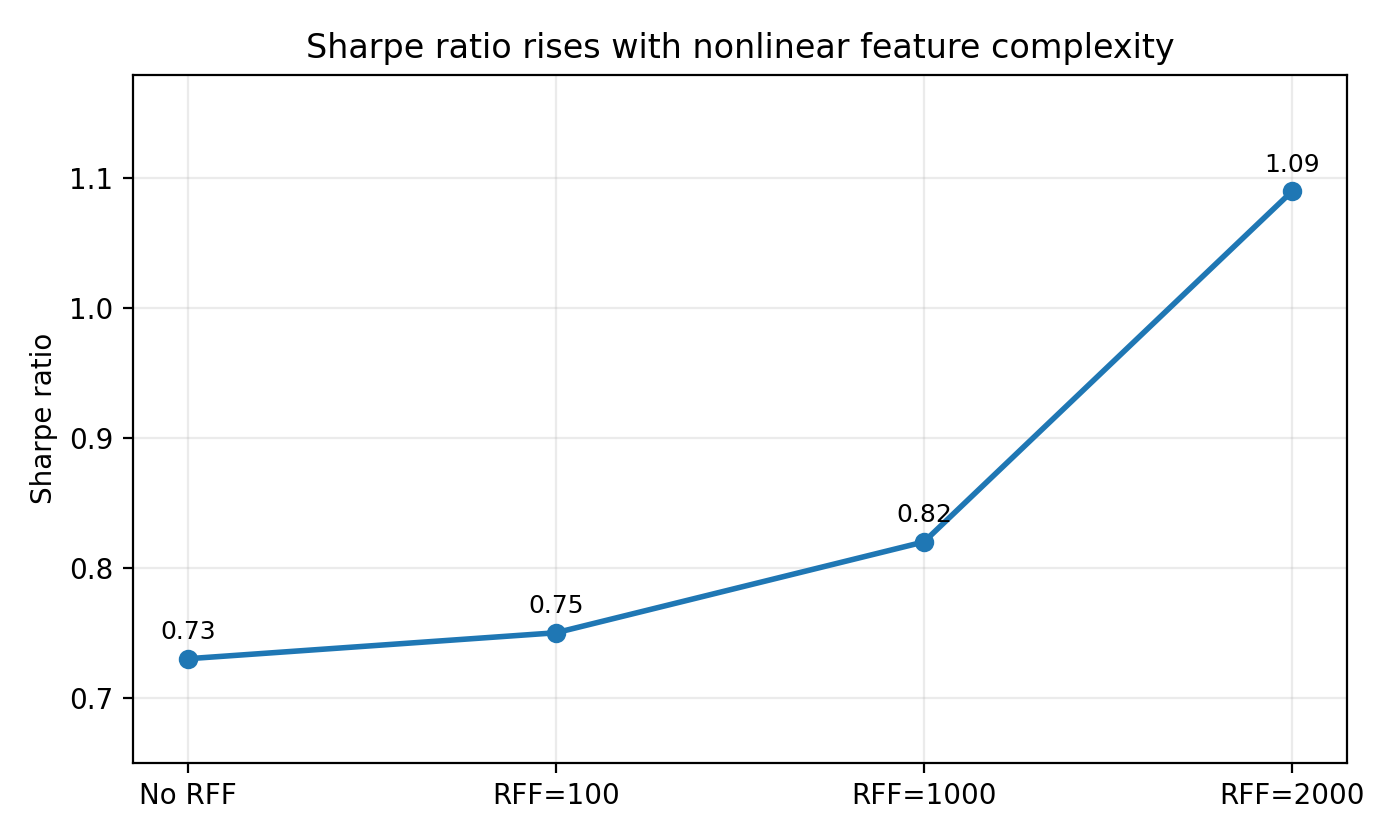
\includegraphics[width=0.78\textwidth]{figures/sharpe_trend.png}
\caption{Sharpe ratio versus model complexity. The upward trend supports the virtue of complexity in portfolio performance.}
\label{fig:sharpe}
\end{figure}

\begin{figure}[H]
\centering
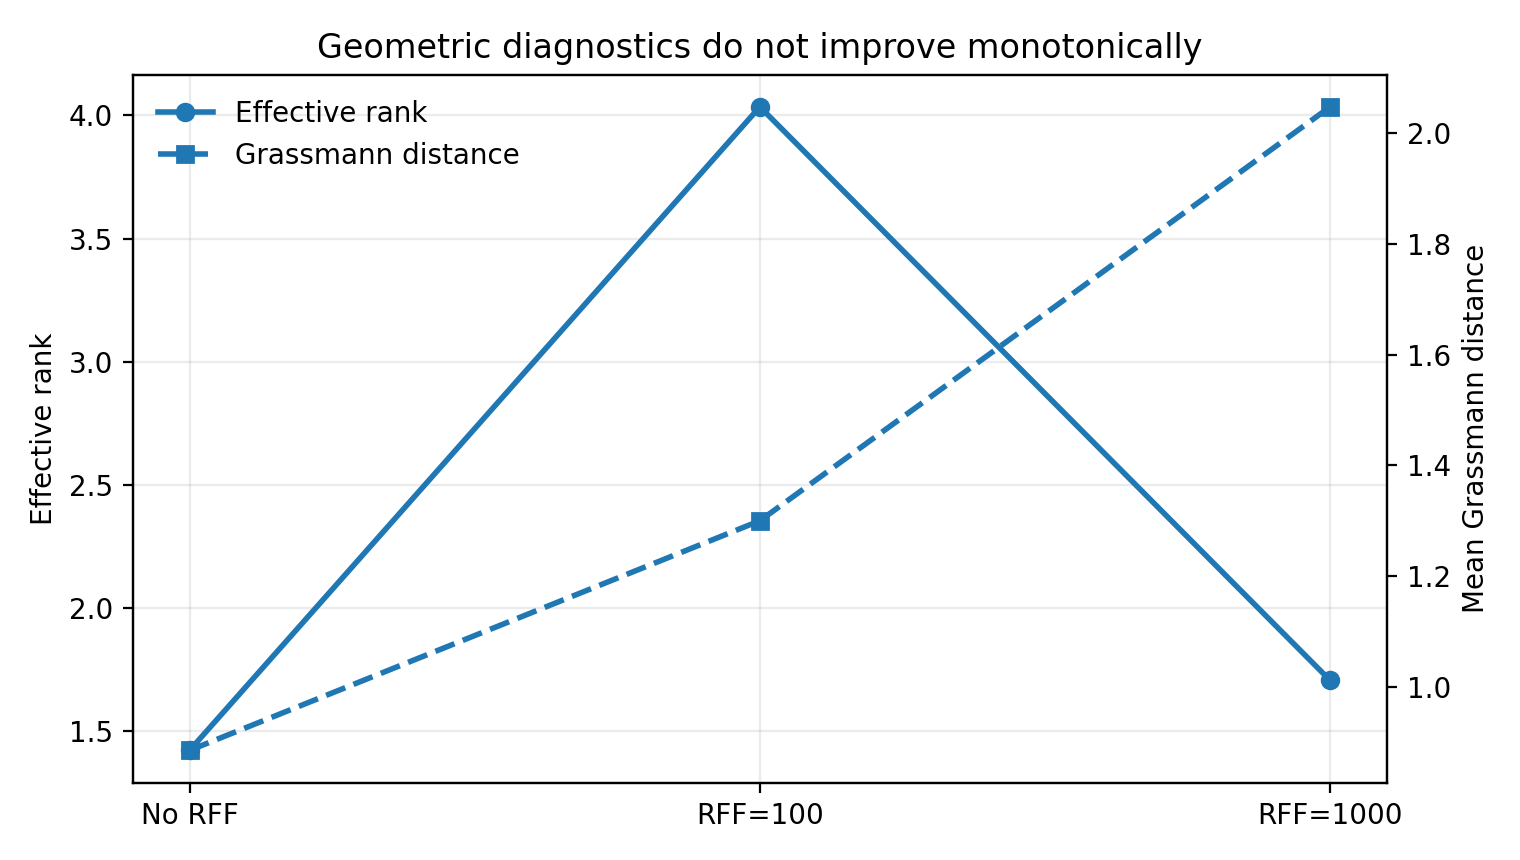
\includegraphics[width=0.82\textwidth]{figures/geometry_summary.png}
\caption{Summary geometric diagnostics. Effective rank and Grassmann distance do not improve monotonically as complexity rises.}
\label{fig:geomsummary}
\end{figure}

\begin{figure}[H]
\centering
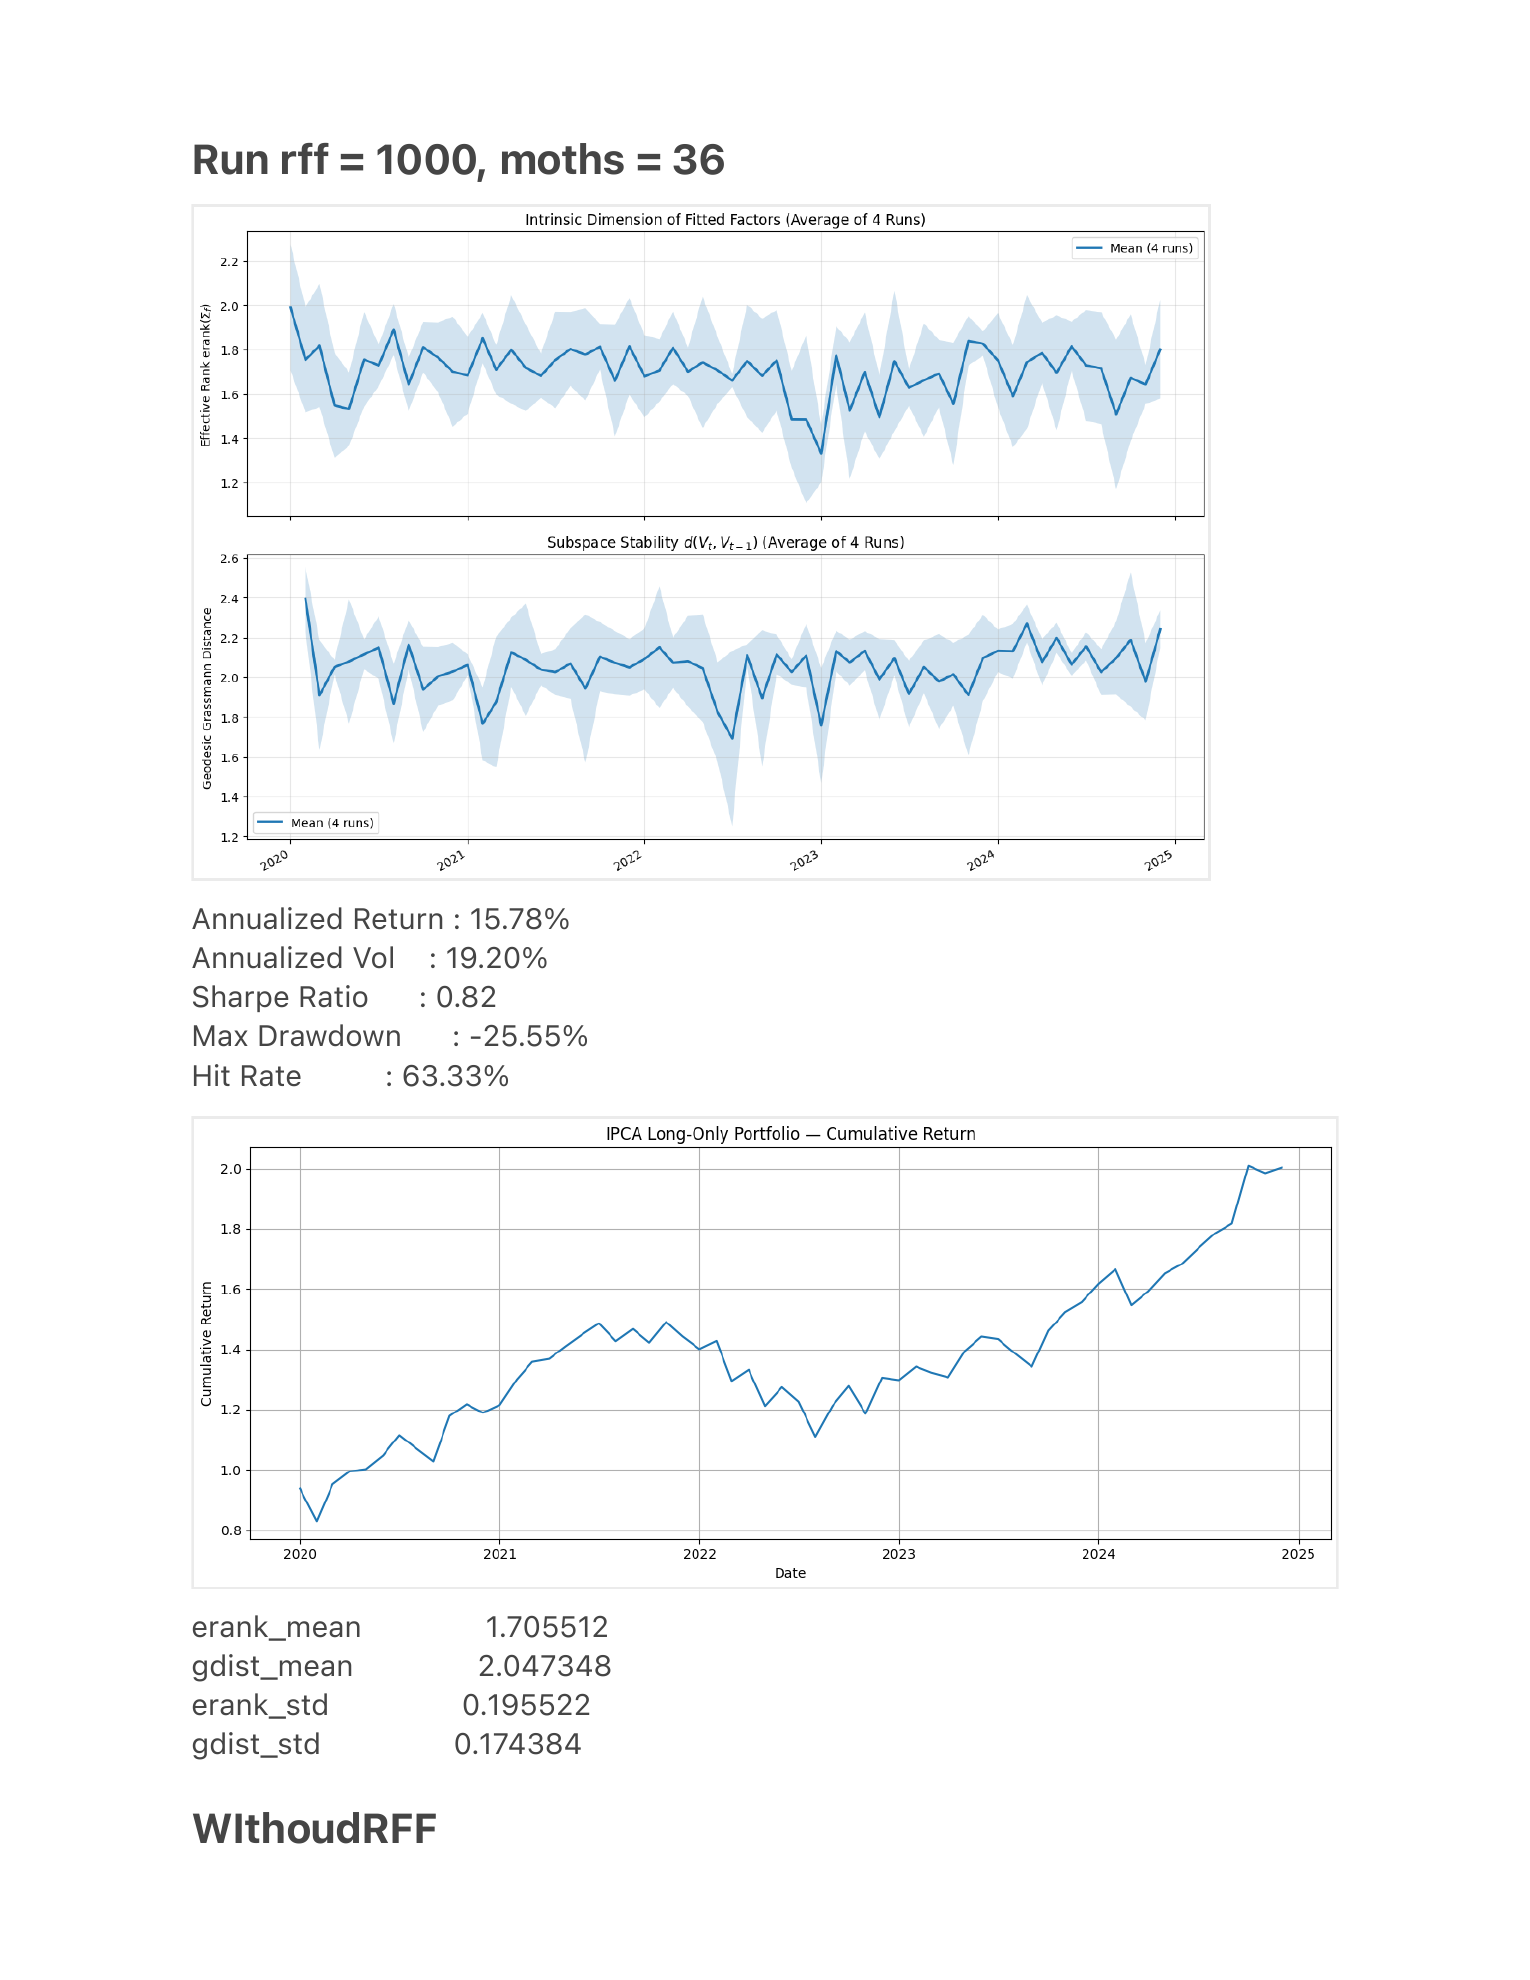
\includegraphics[width=0.88\textwidth]{figures/results_page1.png}
\caption{Extracted panel from the uploaded PDF: RFF = 1000 summary and comparison to the baseline.}
\end{figure}

\begin{figure}[H]
\centering
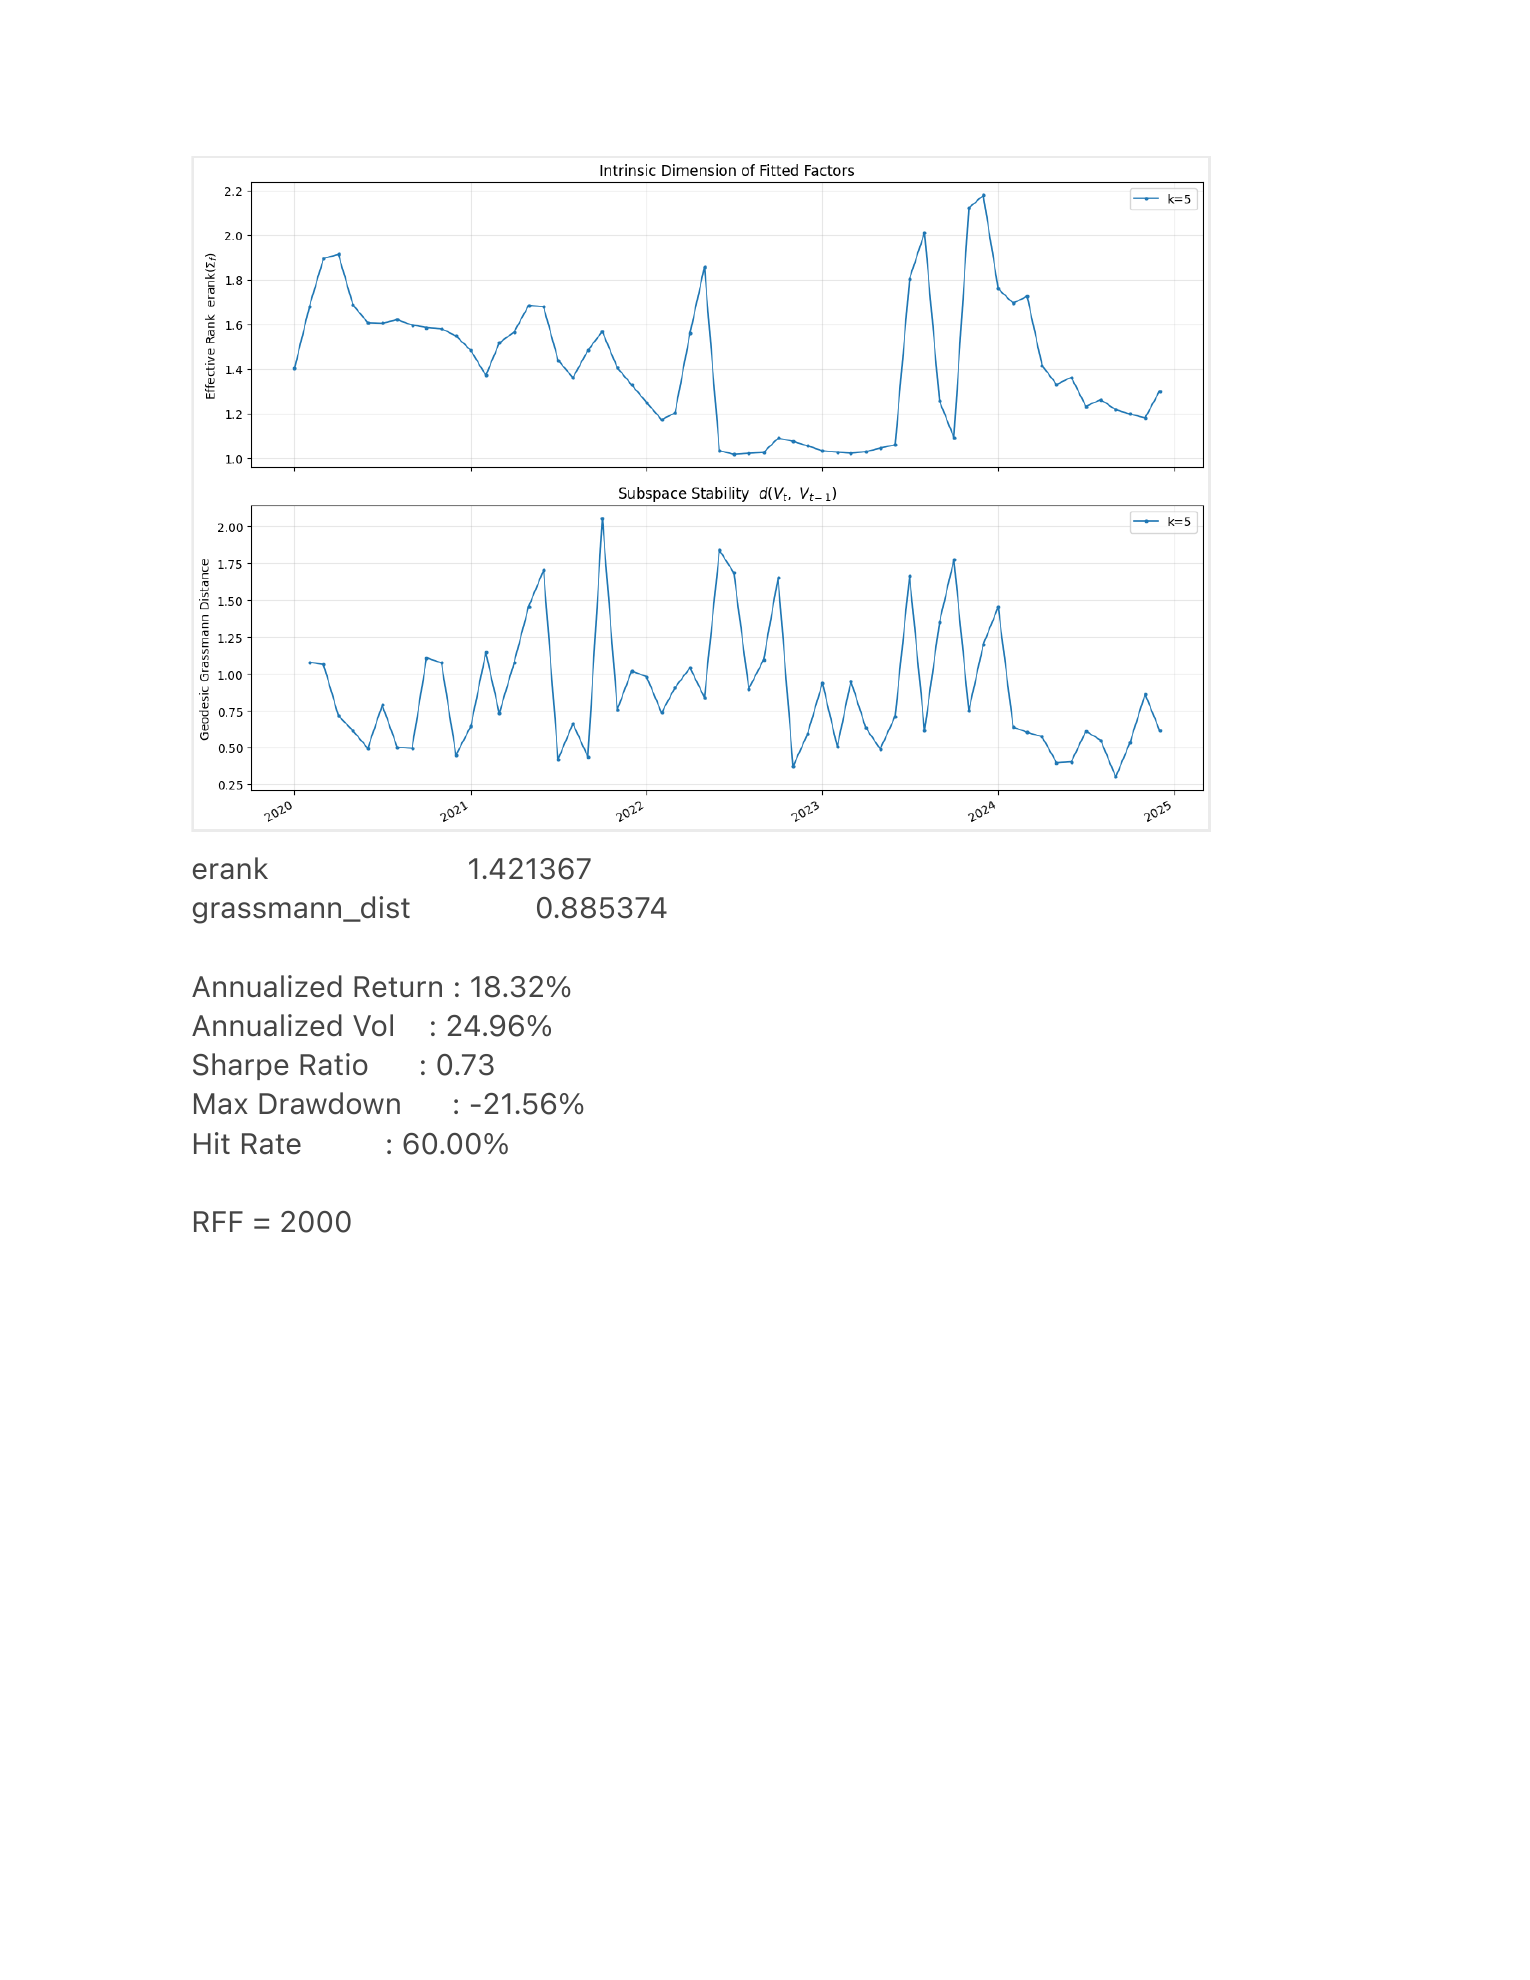
\includegraphics[width=0.88\textwidth]{figures/results_page2.png}
\caption{Extracted panel from the uploaded PDF: baseline / no-RFF summary.}
\end{figure}

\begin{figure}[H]
\centering
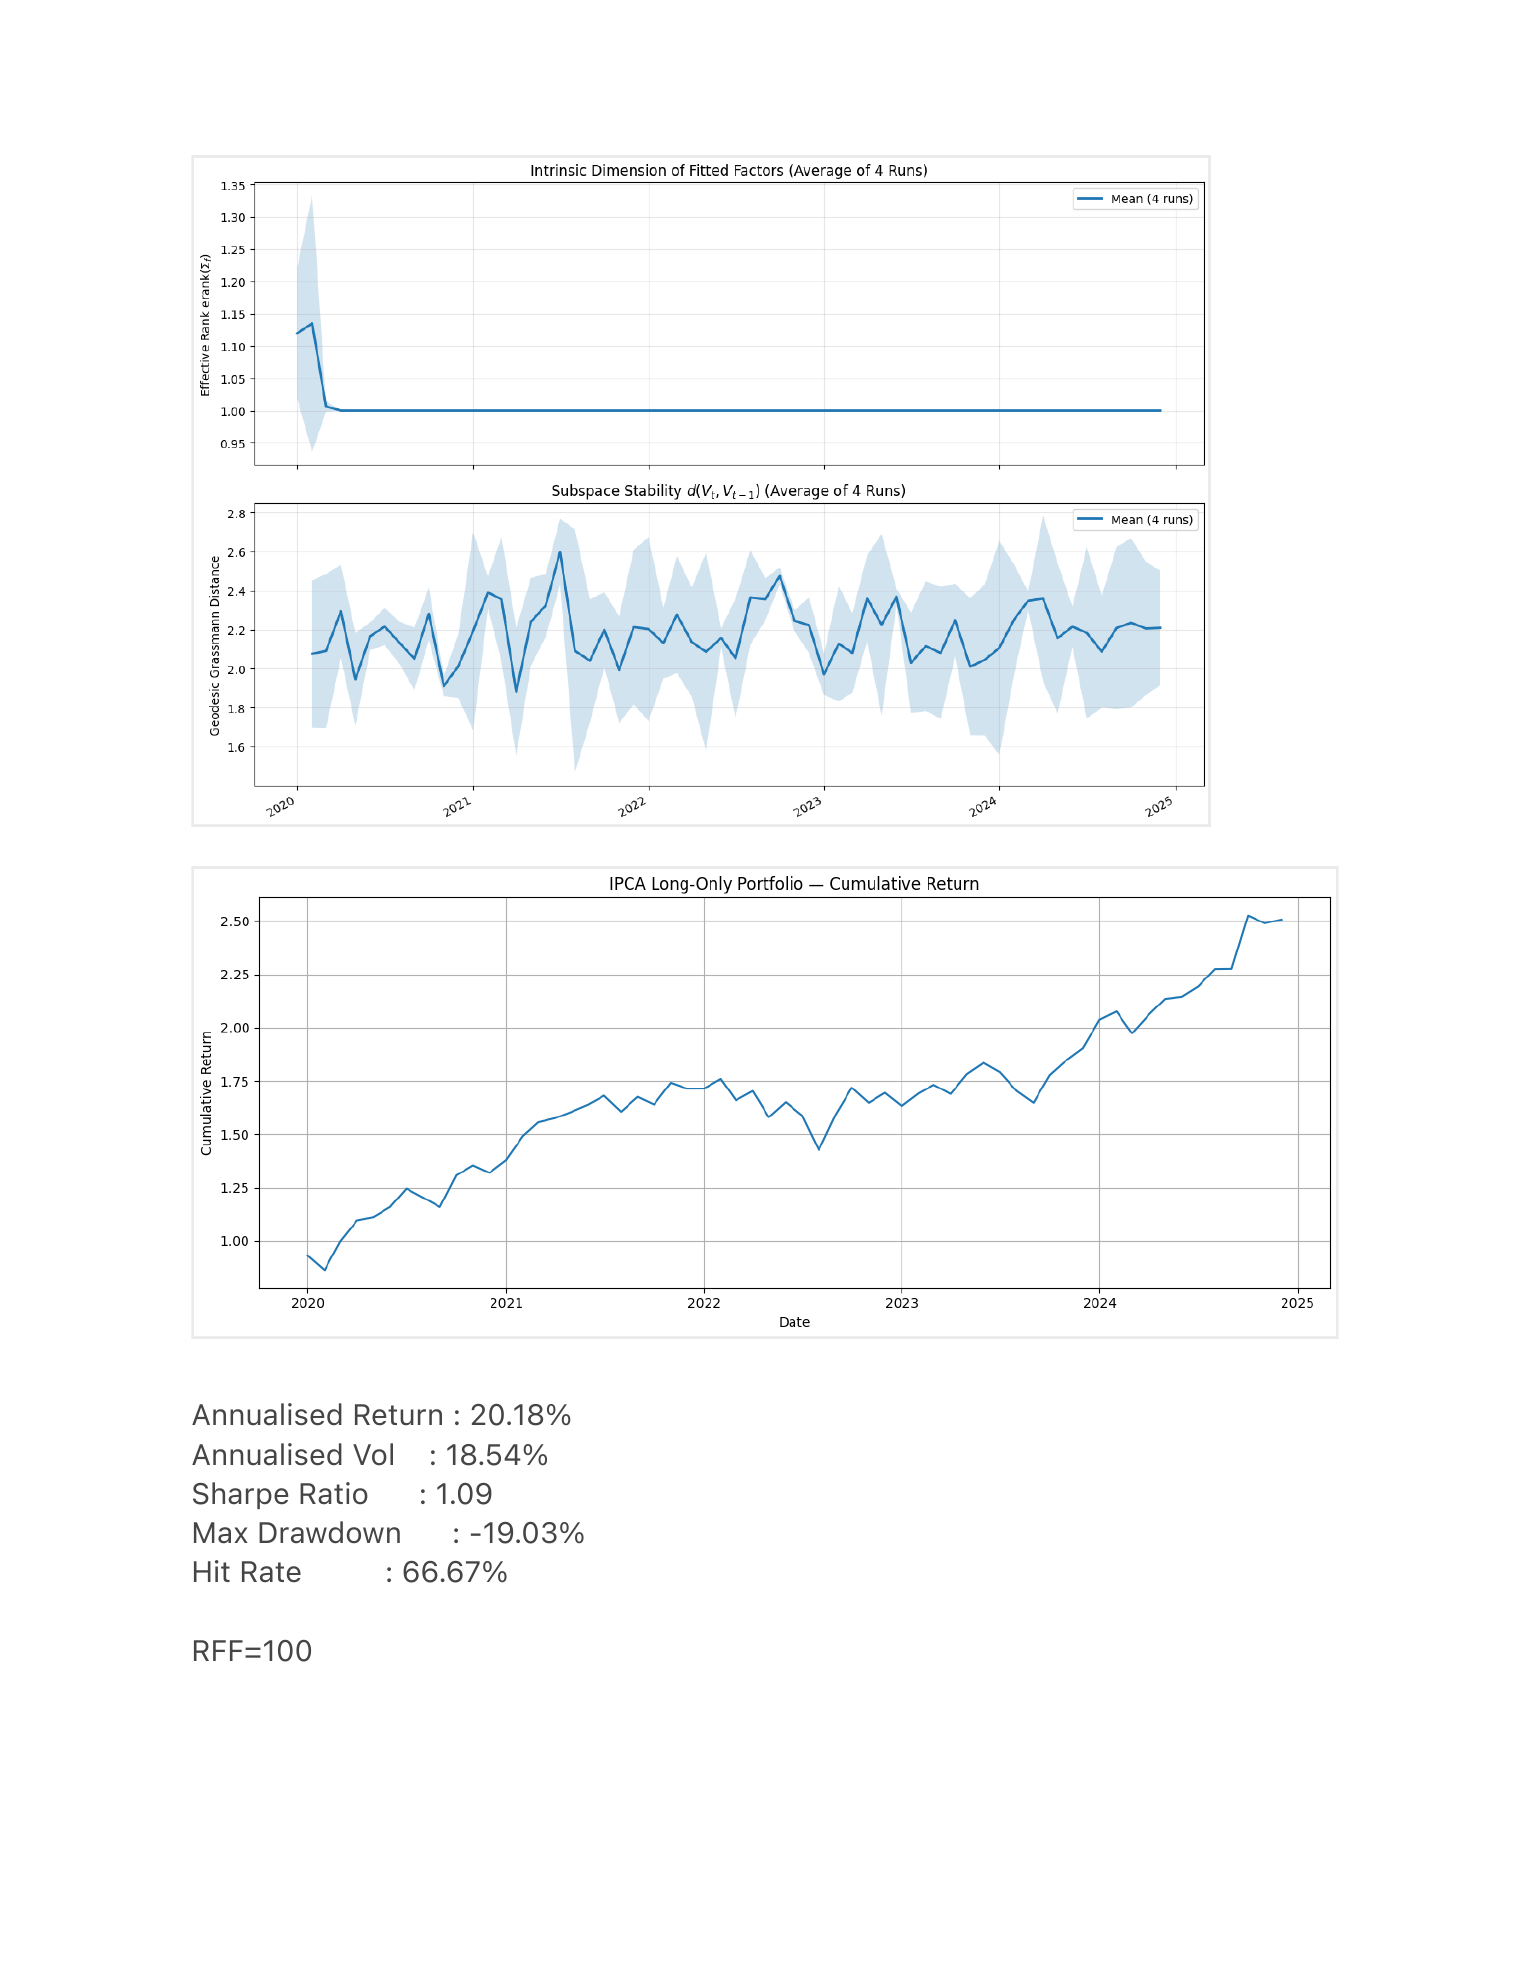
\includegraphics[width=0.88\textwidth]{figures/results_page3.png}
\caption{Extracted panel from the uploaded PDF: RFF = 2000 summary.}
\end{figure}

\begin{figure}[H]
\centering
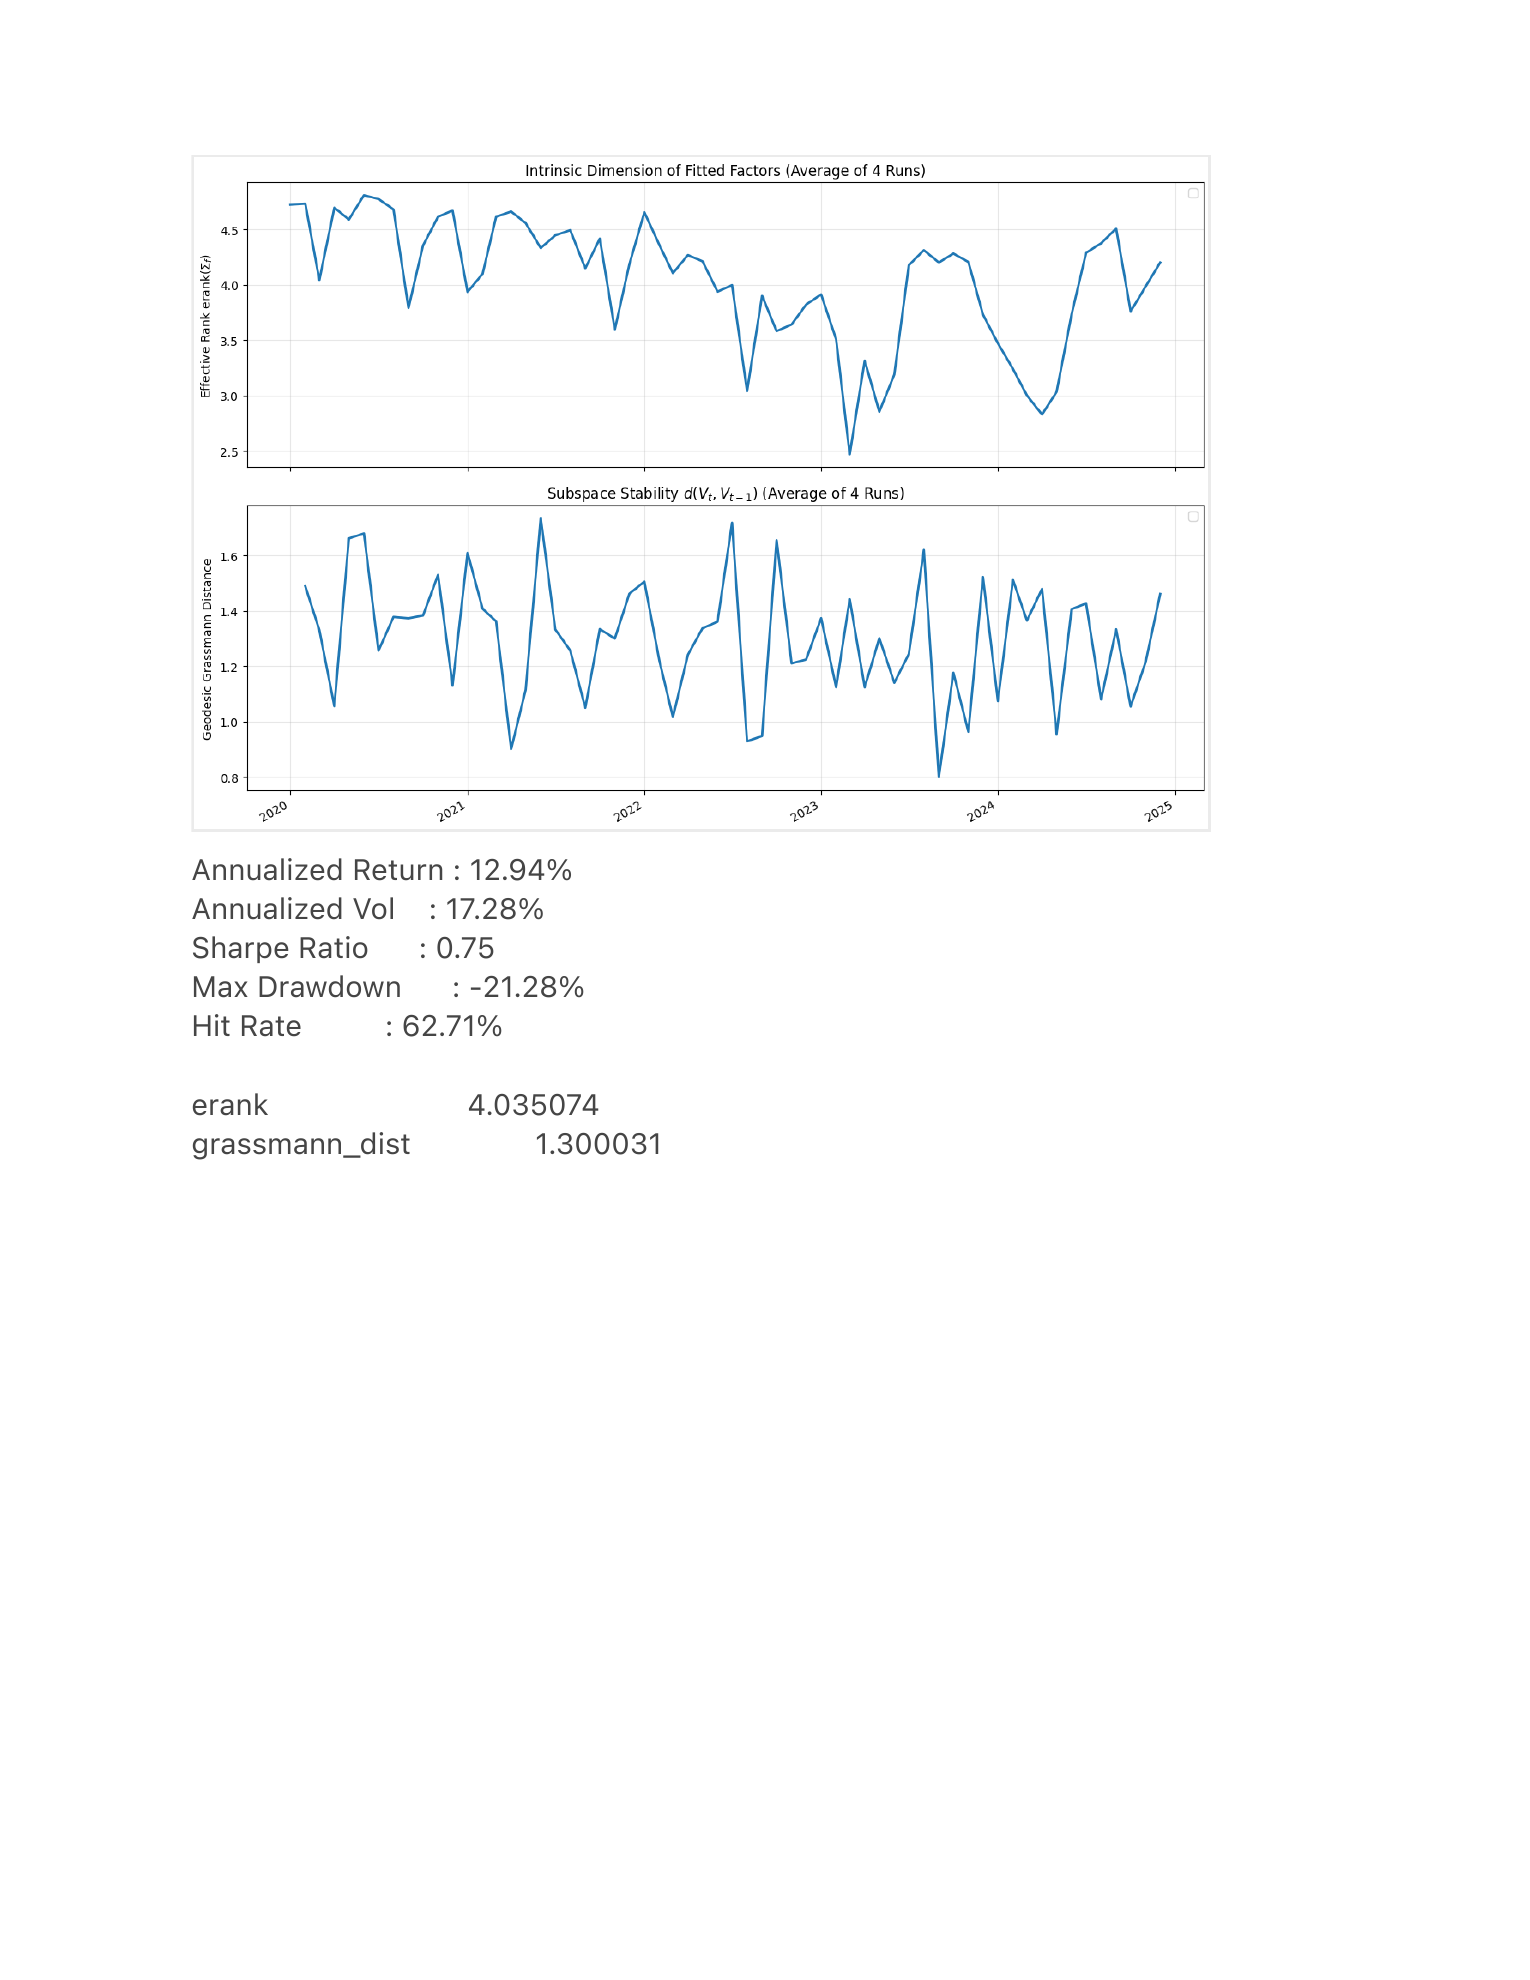
\includegraphics[width=0.88\textwidth]{figures/results_page4.png}
\caption{Extracted panel from the uploaded PDF: RFF = 100 summary.}
\end{figure}
	
\subsection{Rolling-window Grassmann diagnostics}

The strongest geometric evidence comes from the rolling-window plots. These are important because they reveal whether the estimated subspaces are merely fitting well in aggregate, or whether they remain stable through time.

\noindent
\textit{RFF = 1000.} The RFF = 1000 rolling plot is especially useful because it combines the two objects that matter most: effective rank and Grassmann distance. In the uploaded figure, effective rank stays in a fairly narrow band, but Grassmann distance remains elevated. That is evidence of persistent subspace rotation even when performance is decent.

\begin{figure}[H]
\centering
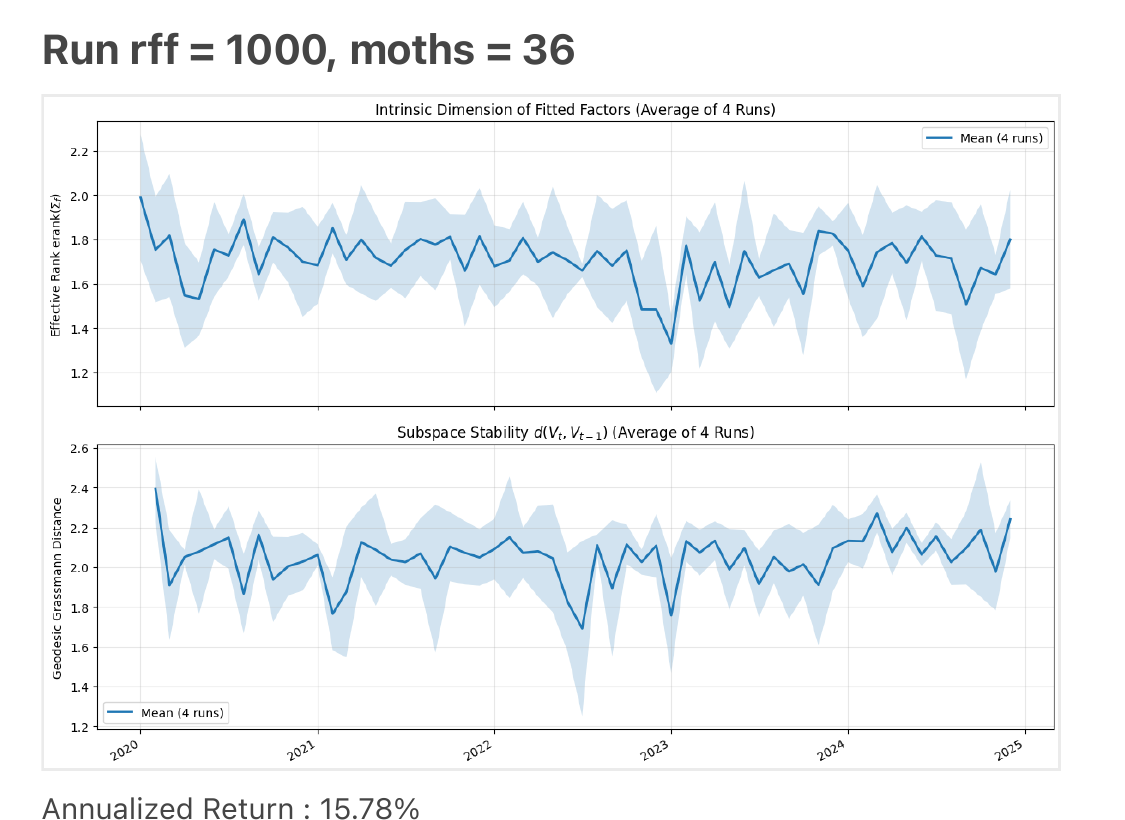
\includegraphics[width=0.96\textwidth]{figures/rff1000_roll.png}
\caption{Rolling effective-rank and Grassmann-distance diagnostics for RFF = 1000. This is the cleanest direct evidence that improved performance does not necessarily imply subspace stability.}
\end{figure}

\begin{figure}[H]
\centering
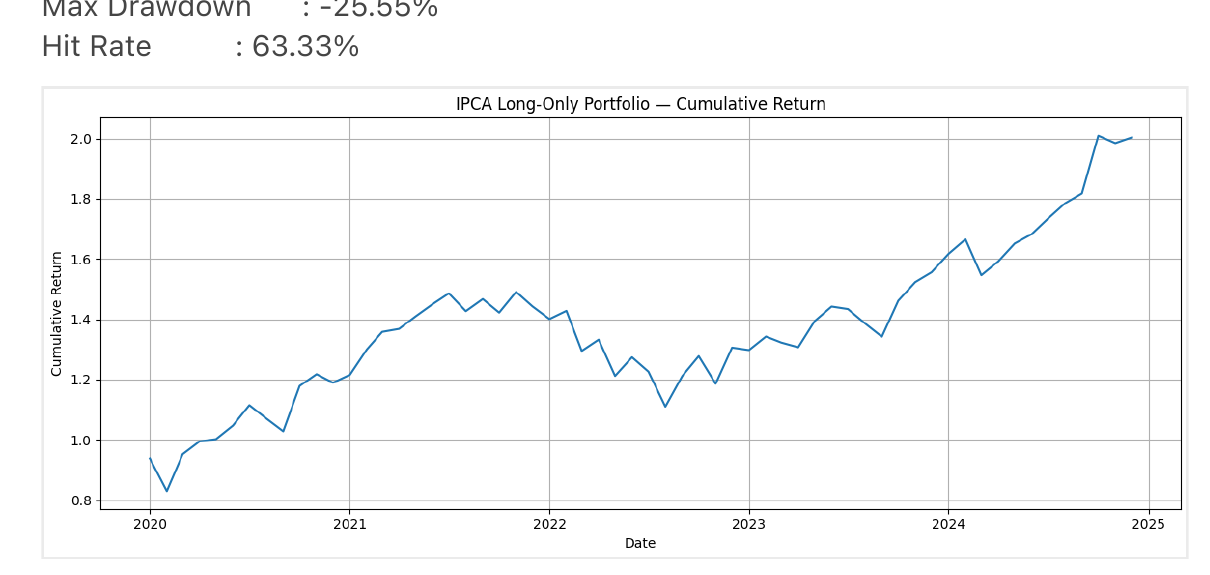
\includegraphics[width=0.78\textwidth]{figures/rff1000_cum.png}
\caption{Cumulative return path for the RFF = 1000 specification. Performance compounds well despite the elevated rolling Grassmann distance.}
\end{figure}

\noindent
\textit{Baseline and lower-complexity comparison.} The next two figures help explain the tradeoff. Without RFF, the system is simpler and Grassmann movement is more limited.
At RFF = 100, effective rank is relatively high, which suggests that the added flexibility is actually spreading across more active directions. By RFF = 1000, however, the span appears less intrinsically rich and more rotationally unstable.

\begin{figure}[H]
\centering
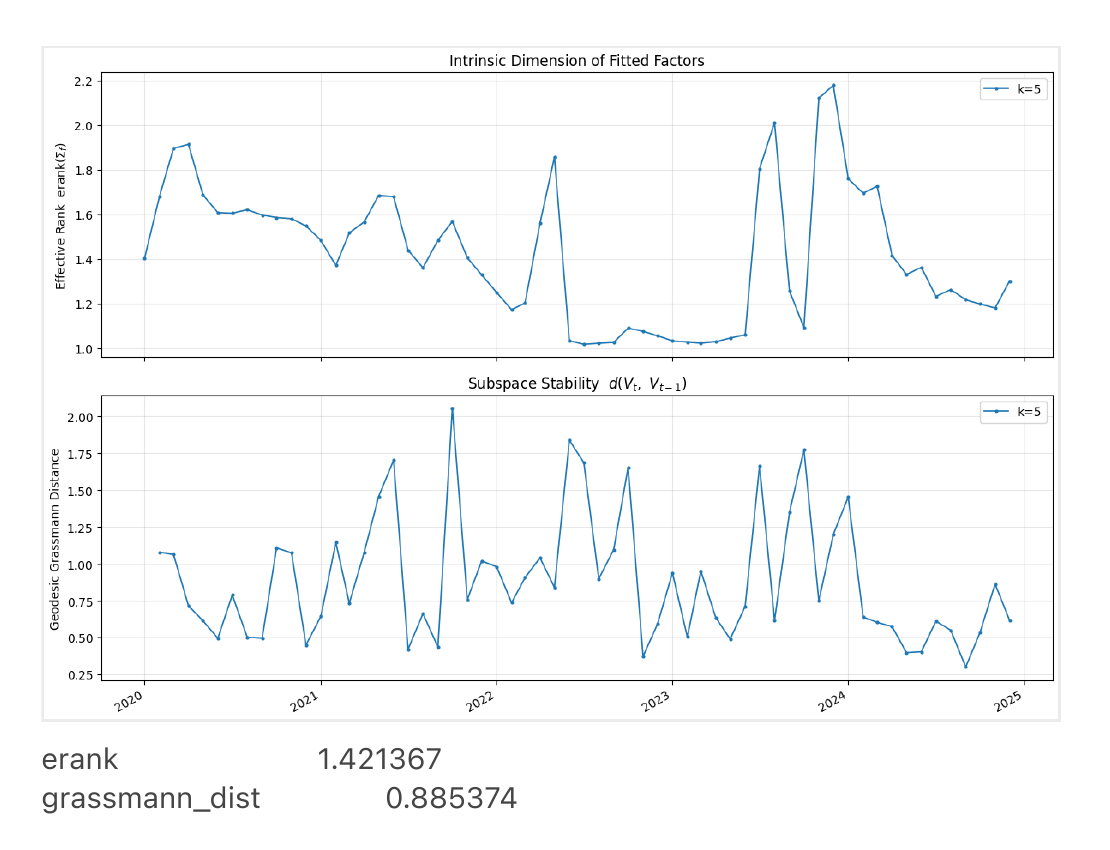
\includegraphics[width=0.95\textwidth]{figures/norrff_roll.png}
\caption{Rolling diagnostics for the no-RFF baseline.}
\end{figure}

\begin{figure}[H]
\centering
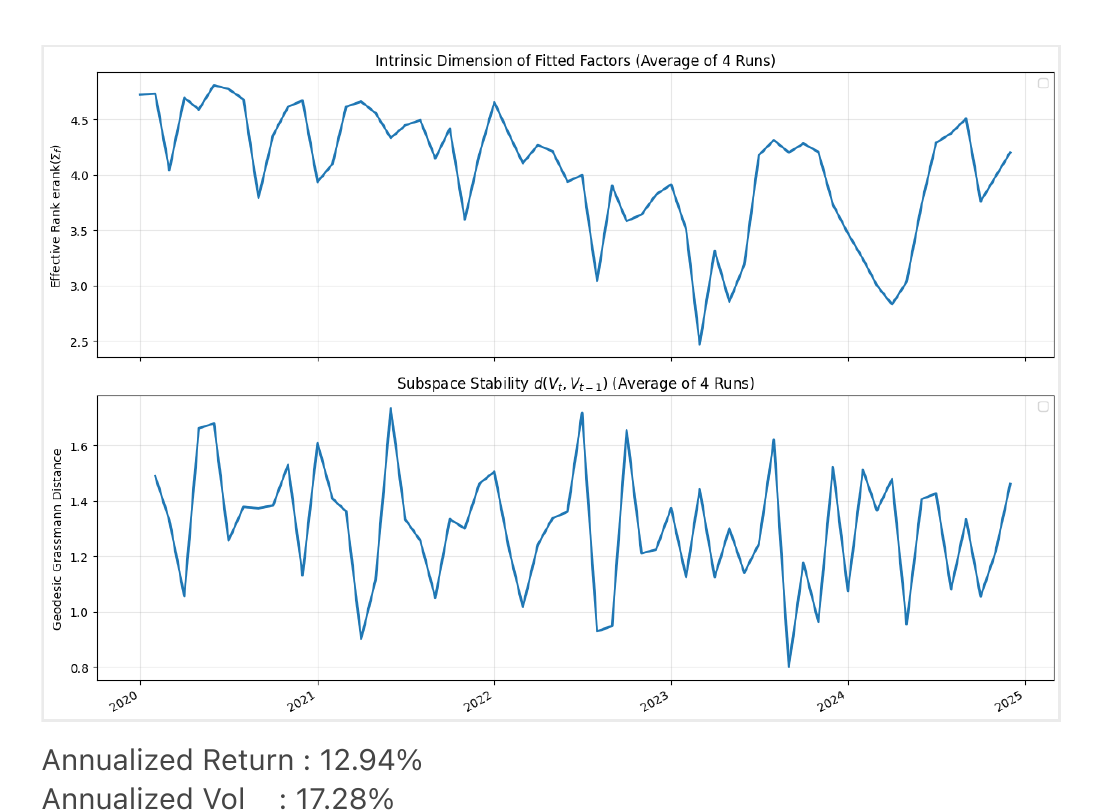
\includegraphics[width=0.95\textwidth]{figures/rff100_roll.png}
\caption{Rolling diagnostics for RFF = 100. This is the configuration with the strongest effective-rank number among the page-level summaries.}
\end{figure}

\begin{figure}[H]
\centering
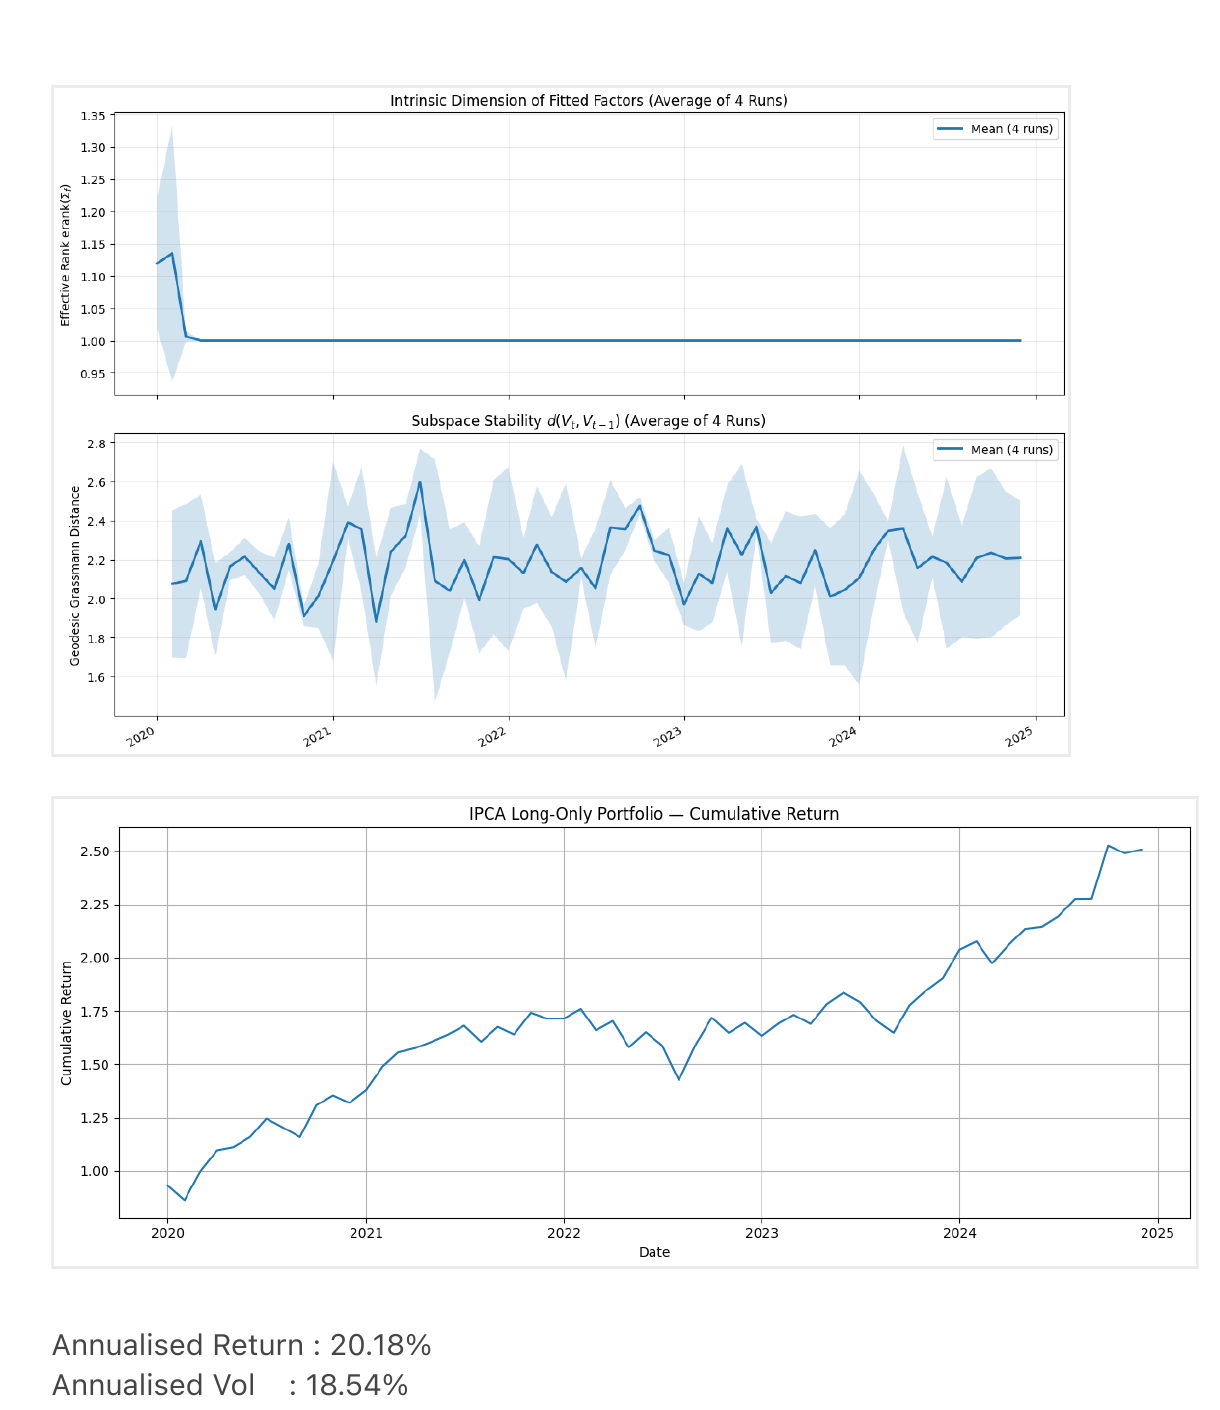
\includegraphics[width=0.95\textwidth]{figures/rff2000_roll_cum.png}
\caption{High-complexity panel for RFF = 2000. This configuration has the strongest Sharpe ratio in the summary results.}
\end{figure}
	
\subsection{Supplementary comparison pages}
	
The remaining two figures are useful as compact references because they place multiple configurations side by side.

\begin{figure}[H]
\centering
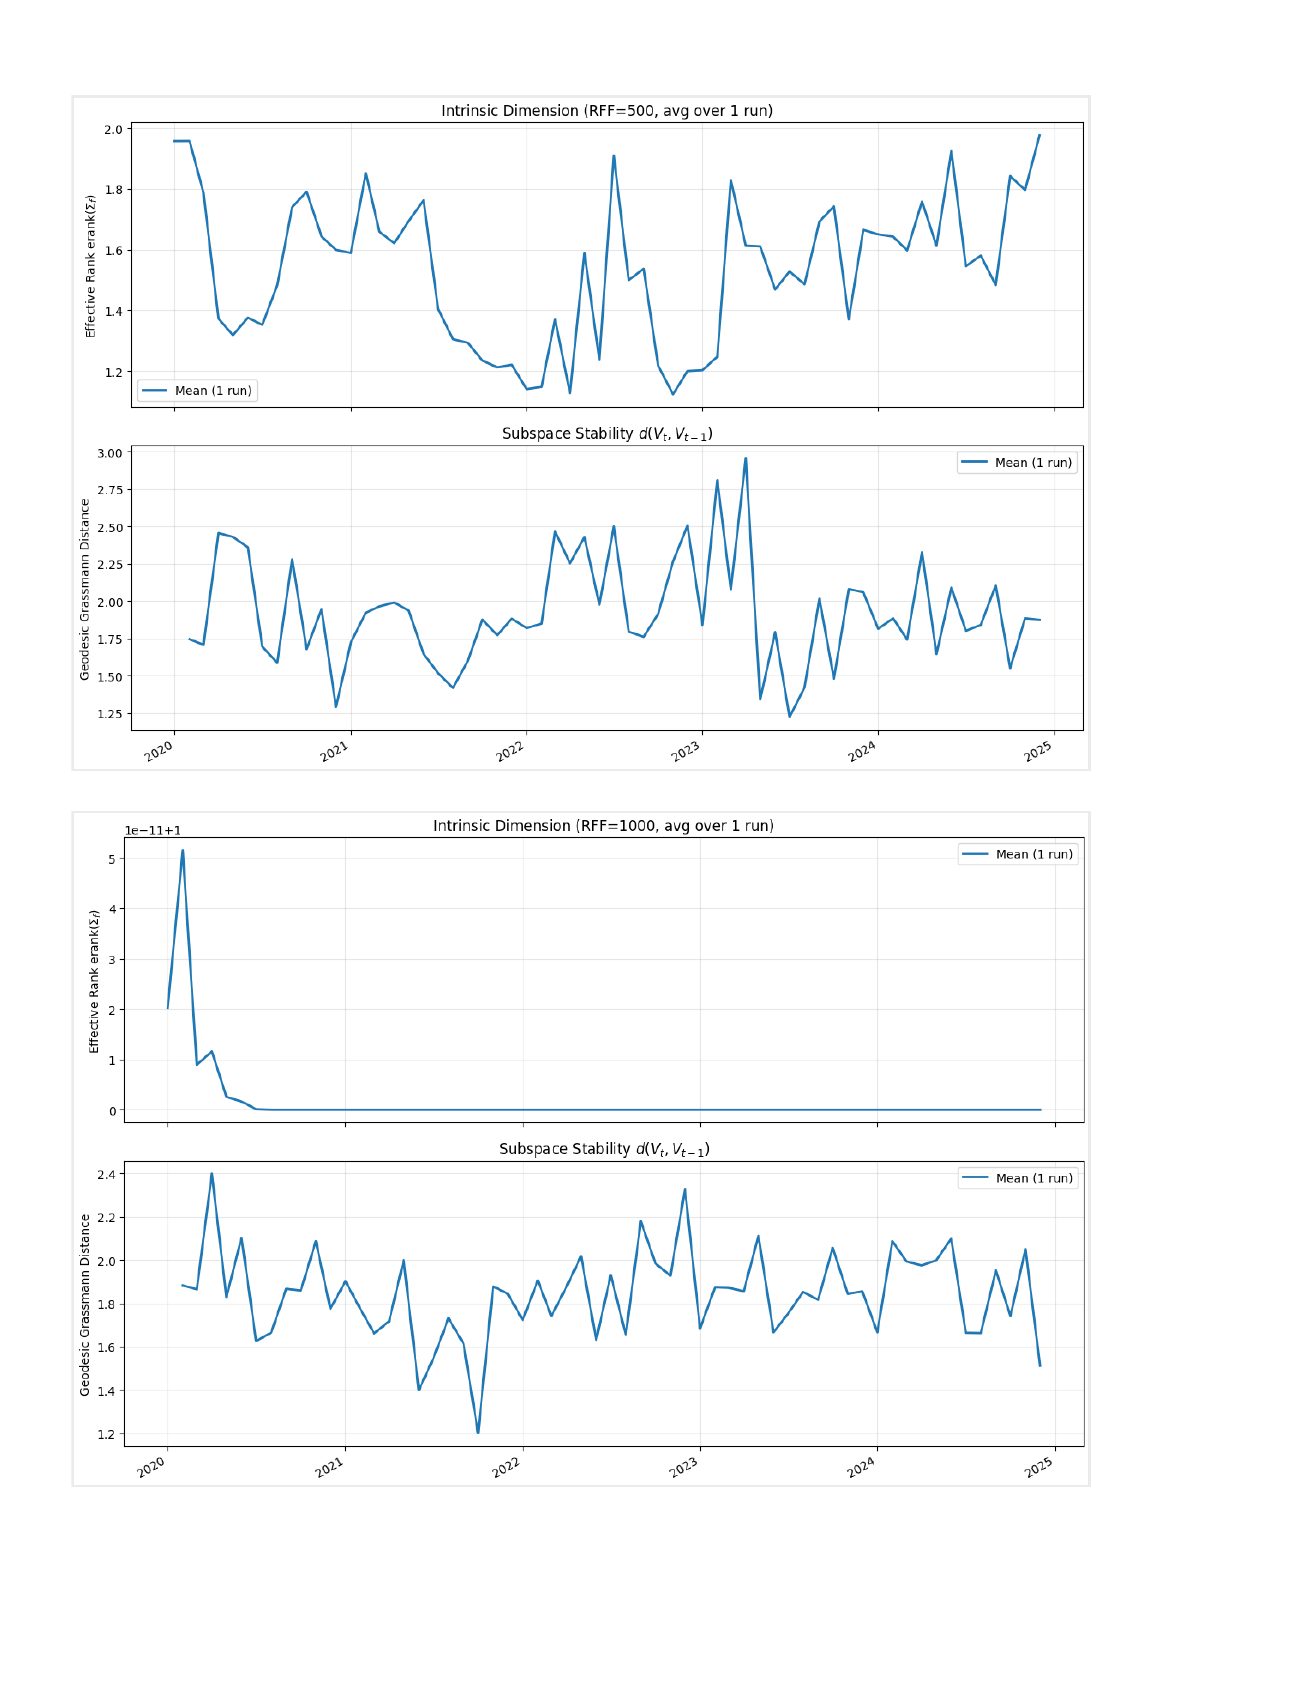
\includegraphics[width=0.96\textwidth]{figures/compare_500_1000.png}
\caption{Side-by-side comparison page for RFF = 500 and RFF = 1000.}
\end{figure}

\begin{figure}[H]
\centering
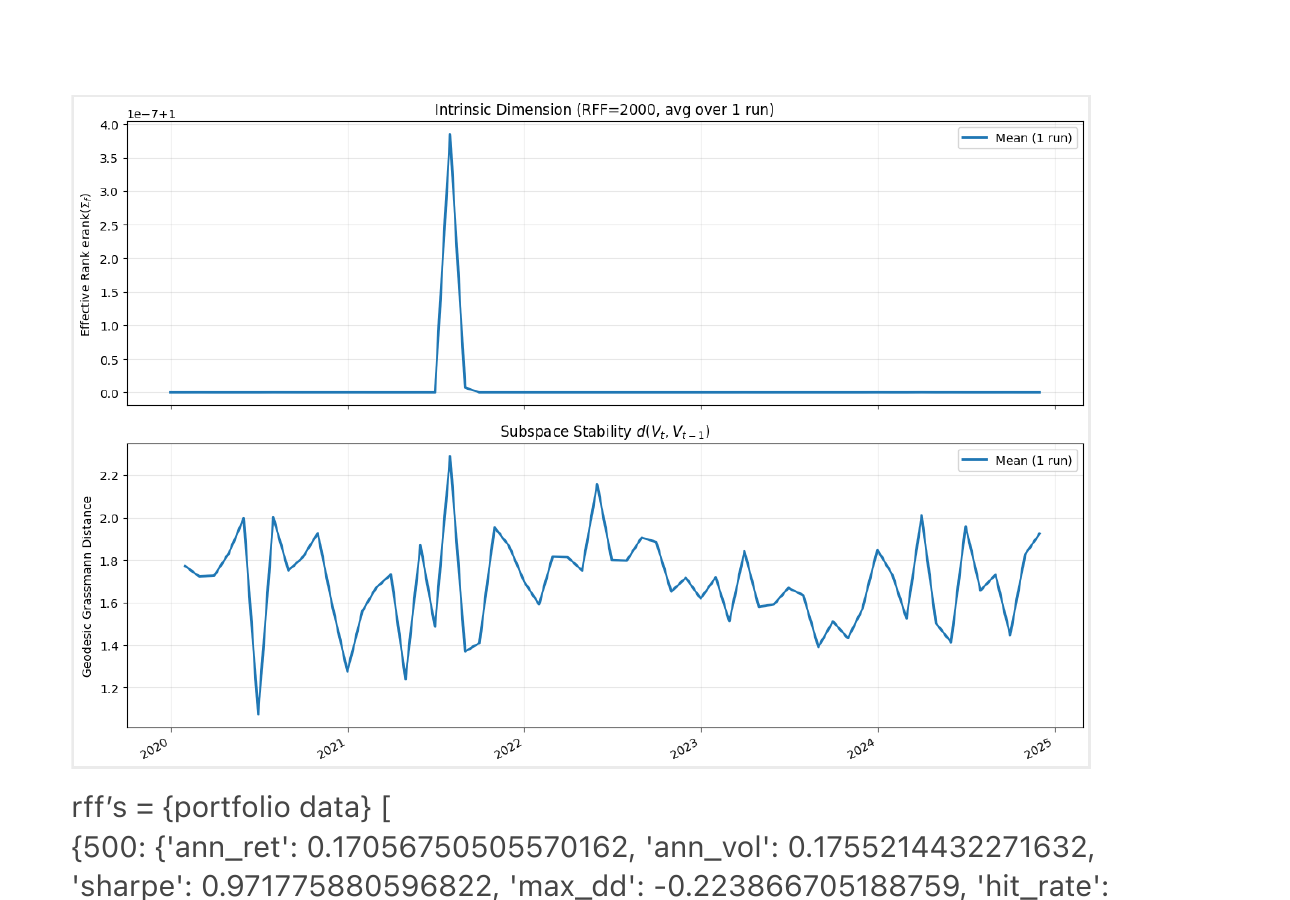
\includegraphics[width=0.96\textwidth]{figures/compare_2000_summary.png}
\caption{One-run summary page for RFF = 2000.}
\end{figure}

\subsubsection{Connection to the Virtue of Complexity}

The uploaded results are aligned with the broad message of the virtue-of-complexity literature. Higher nonlinear complexity can improve out-of-sample Sharpe ratio because it expands approximation power and allows the model to capture richer conditional structure than a linear or low-dimensional alternative.

So on the \emph{performance} dimension, the evidence is straightforward:
\begin{itemize}
\item No RFF: Sharpe $\approx 0.73$
\item RFF = 100: Sharpe $\approx 0.75$
\item RFF = 1000: Sharpe $\approx 0.82$
\item RFF = 2000: Sharpe $\approx 1.09$
\end{itemize}

That progression is difficult to dismiss. It says the nonlinear lifting is economically valuable.
	
\subsection{Connection to Grassmann geometry}

The geometry paper introduces a different standard for evaluating complexity.
The issue is not only whether richer models fit or trade better, but whether they identify a \emph{stable} and \emph{persistent}
trajectory of return subspaces.

Under that lens, the evidence here is more mixed:
\begin{itemize}
\item effective rank is not monotone in complexity,
\item rolling Grassmann distance can increase materially,
\item the strongest performance setting may still be geometrically unstable.
\end{itemize}

This means some of the additional nonlinear flexibility may be \emph{structurally meaningful}, while some may be \emph{illusory}:
it improves fit or trading performance, but through directions that are weakly identified and rotate under perturbation.

\subsection{IPCA versus Grassmann Framework}

Standard IPCA estimates a parameter matrix and latent factors through a least-squares criterion. In a high-dimensional lifted feature space, that creates a serious identification problem. Namely,
\begin{itemize}
\item[(i)] many different parameter matrices can induce nearly the same fitted return span,
\item[(ii)] the objective function becomes flat in directions that rotate the span inside weakly identified eigenspaces,
\item[(iii)] optimization can therefore look numerically successful while the underlying parameterization remains unstable.
\end{itemize}
In other words, the estimator is solving for the wrong object. The economically meaningful object is the induced return span, not the raw loading matrix.

That is exactly why the rolling Grassmann plots are so useful. They show that even when cumulative returns look good, the subspaces can still move around materially. So the issue is not that IPCA cannot produce a fit. It clearly can. The issue is that in this regime the fitted coefficients are not the right thing to interpret or stabilize. In other words, in a high-dimensional RFF lift, standard Kelley IPCA can be economically successful but geometrically unstable.
That makes it a poor estimator for ``stable IPCA'' even when its out-of-sample Sharpe ratio looks strong.
		
A Grassmann-based framing asks for three diagnostics jointly:
\begin{itemize}
\item[(i)] out-of-sample performance,
\item[(ii)] intrinsic dimension (effective rank),
\item[(iii)] rolling subspace stability (Grassmann distance).
\end{itemize}
That combined view is much stronger than using Sharpe alone. It lets you say:
\begin{itemize}
\item[(i)] complexity is \textit{economically virtuous} when Sharpe improves,
\item[(ii)] complexity is \textit{geometrically virtuous} only when that improvement comes with persistent, stable span expansion.
\end{itemize}

The results of thie section support the first statement strongly, but support the second only partially. That is exactly why a Grassmann estimator or a Grassmann comparison framework is more defensible than a raw IPCA coefficient analysis. The RFF-IPCA results support the virtue of complexity in portfolio performance, but the rolling Grassmann plots show that the added nonlinear flexibility does not uniformly stabilize the identified return span; therefore standard IPCA is not a good choice when the goal is stable IPCA in a lifted-feature regime.


\section{Historical Data Analysis: Neural Network Models}

In the Geometry of Complexity perspective, the relevant object is not the raw number of parameters but the stability of the span of predictive return signals. In financial prediction problems with weak signals and limited samples, models that add flexibility must do so in a way that expands the signal span while preserving stability across rolling estimation windows.

% ----------------------------
\subsection{Empirical Findings from the LSTM Experiments.}

In the LSTM backtests replacing Random Fourier Features, two complexity controls were varied: Hidden layers (depth) and Hidden dimensions (width). The observed pattern was: Increasing layers increased Sharpe ratio and mean return while reducing volatility. Increasing hidden dimensions produced the opposite effect: Sharpe declined and volatility increased. This suggests that different forms of complexity influence the learned return signal space differently.

% ----------------------------
\subsection{Connection to the RFF (Kelly-Malamud-Zhou) Experiments.}

Earlier experiments using Random Fourier Features showed stronger performance with lower values of the kernel parameter $\gamma$. A lower $\gamma$ produces smoother feature maps, effectively limiting the number of independent directions introduced by the nonlinear transformation. Geometrically, this prevents the model from creating many weak, sample-specific directions in return space. The LSTM results appear consistent with this principle: architectures that introduce complexity in a structured manner (such as additional layers) improve stability, while those that primarily increase parameter dimensionality (large hidden dimensions) may create unstable directions that degrade risk-adjusted performance.

% ----------------------------
\subsection{Understanding Hidden Layers vs Hidden Dimensions.}

The diagram below illustrates the conceptual difference between depth and width in an LSTM architecture. Each column represents a layer of the network, while each dot represents a hidden unit within that layer.

\begin{figure}[h]
\centering
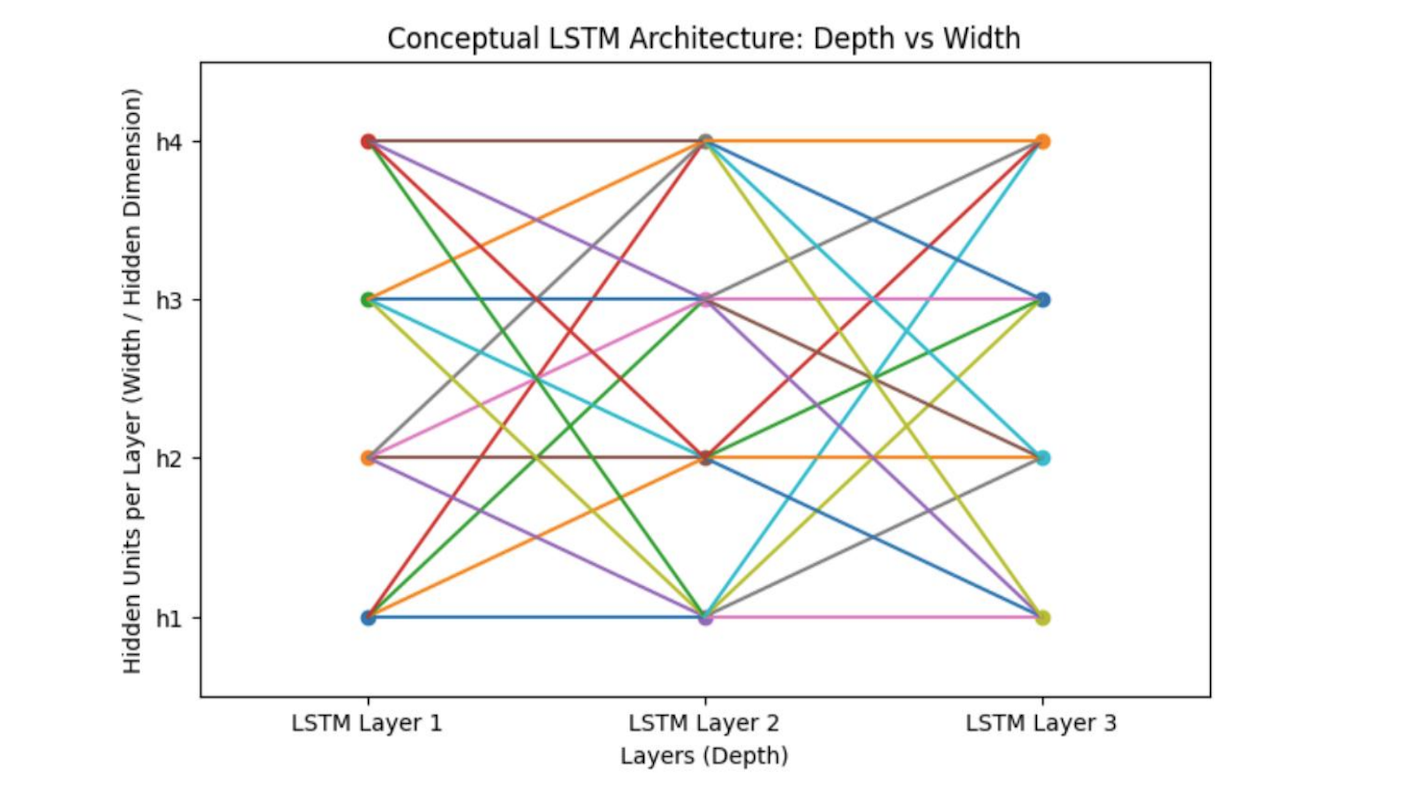
\includegraphics[width=0.85\textwidth]{diagram.png}
\end{figure}

\subsection{Hidden Dimensions (Width)}

Increasing hidden dimensions increases the number of hidden units within a layer. This dramatically increases the number of parameters and the number of possible directions the model can represent. While this increases expressive power, it may also introduce directions that are weakly identified in finite samples. When the model is retrained in rolling windows, these weak directions can rotate with sampling noise, leading to unstable forecasts and higher volatility.

\subsection{Hidden Layers (Depth)}

Increasing layers adds hierarchical transformations rather than simply adding independent directions. Each layer can refine temporal patterns detected by previous layers, effectively creating structured filters over time. This often improves the alignment of the learned representation with persistent components of the return signal space. As a result, deeper architectures may expand the effective signal span more stably than wider architectures.

\section{Conclusion}

The debate over the ``virtue of complexity'' in asset pricing is fundamentally geometric. Nonlinear exposure maps may expand parameter dimension without expanding intrinsic return dimension.

The economically relevant object is the return subspace. Grassmann geometry provides tools to measure intrinsic dimension, stability, and curvature.

Reframing the debate in geometric terms clarifies when complexity reflects structural discovery and when it reflects statistical illusion. 

These results support the broader Geometry of Complexity idea: the useful notion of complexity is not the number of parameters but the stability and effective dimensionality of the learned return signal subspace. Complexity that expands the signal span smoothly (e.g., deeper architectures or smoother feature maps) tends to improve Sharpe ratios, while complexity that mainly increases parameter dimensionality may introduce unstable directions and degrade performance.

\medskip\noindent
\textbf{Declaration of generative AI and AI-assisted technologies in the manuscript preparation process}: During the preparation of this work, the authors used ChatGPT (OpenAI) for language editing and stylistic refinement of portions of the manuscript. All substantive ideas, models, derivations, and conclusions are solely those of the author. After using this tool, the authors reviewed and edited the content as needed and takes full responsibility for the content of the published article.

\begin{thebibliography}{99}
\bibitem{AMS08} Absil, P.-A., Mahony, R., and Sepulchre, R.: \emph{Optimization Algorithms on Matrix Manifolds}, Princeton University Press, (2008).
\bibitem{BZA24} Bendokat, T., Zimmermann, R., and Absil, P.-A.:  A Grassmann manifold handbook: basic geometry and computational aspects, \emph{Advances in Computational Mathematics}, \textbf{50}, 6 (2024).
\bibitem{B97} Bhatia, R.: \emph{Matrix Analysis}, Springer Verlag (1997).
\bibitem{GW08} Goyal, A., and Welch, I.: A comprehensive look at the empirical performance of equity premium prediction, \textit{Review of Financial Studies}, \textbf{21}, 1455 - 1508 (2008).
\bibitem{KM25} Kelly, B., and Malamud, S.: Understanding the Virtue of Complexity, SSRN 5346842 (2025).
\bibitem{KPS19} Kelly, B., Pruitt, S., and Su, Y.: Characteristics are Covariances: A Unified Model of Risk and Return, \emph{Journal of Financial Economics}, \textbf{134}, 501 - 524 (2019).
\bibitem{KMZ21} Kelly, B., Malamud, S. and Zhou, K.: The Virtue of Complexity in Return Prediction, \textit{The Journal of Finance}, \textbf{79}, 459 - 503 (2024).
\bibitem{LM26} Lesniewski, A., and Missaoui, O.: IPCA and GIPCA via Grassmann optimization (2026).
\bibitem{RR07} Rahimi, A., and Recht, B.: Random Features for Large-Scale Kernel Machines, \textit{Advances in neural information processing systems}, \textbf{20} (2007).
\bibitem{RR08} Rahimi, A., and Recht, B.: Weighted sums of random kitchen sinks: Replacing minimization with randomization in learning, \textit{Advances in neural information processing systems}, \textbf{21} (2008)
\bibitem{RV07} Roy, O., and Vetterli, M.: The effective rank: A measure of effective dimensionality, \emph{2007 15th European Signal Processing Conference}, 606 - 610, Poznan, Poland, (2007).
\end{thebibliography}

\bigskip\noindent
\textbf{Keywords:} Asset pricing, conditional factor models, Grassmann manifold, intrinsic dimension, model complexity, machine learning.

\end{document}